\chapter{RESULTADOS E DISCUSS\~AO}
\label{cap:capitulo4}

\section{Desempenho dos modelos}
%Apresentar e comparar os resultados dos diferentes modelos utilizados.

Os resultados obtidos pelos modelos apresentaram variações significativas em termos de precisão, tanto nas previsões pontuais quanto nos intervalos de confiança, refletindo diferentes graus de precisão para cada cenário analisado. A análise dos resíduos revelou-se particularmente interessante, pois evidenciou comportamentos distintos em função da sazonalidade, com variações marcantes observadas em diferentes períodos do ano.

\subsection{Rio Jequitinhonha}

Iniciando pela menor bacia hidrográfica estudada, os resultados revelaram-se bastante satisfatórios, especialmente no que se refere ao modelo de Regressão Linear, que se destacou com previsões precisas, tanto em termos pontuais quanto nos intervalos de confiança. Este modelo demonstrou uma capacidade robusta de capturar a dinâmica hidrológica do rio, refletindo precisão nas métricas e desempenho consistente, aliado a um tempo de execução significativamente reduzido. Em contrapartida, o modelo (simples) SeasonalNaive apresentou resultados abaixo das expectativas em todas as situações avaliadas. (figura \ref{fig:jequiti_SN_WFV})

Com a MAPE extremamente elevada, de 150\%, os resultados indicaram um viés significativo de superestimação, conforme evidenciado pela métrica PBIAS. Verificando a KGE, ficou negativa. Em outras palavras, isso significa que o modelo não apenas falha em capturar a variabilidade dos dados observados, mas também introduz erros que o tornam menos eficaz do que uma abordagem simplista, como utiilizar a média histórica. Embora a análise superficial da qualidade dos intervalos de confiança pudesse sugerir um desempenho satisfatório do modelo, uma inspeção mais detalhada revela uma incongruência: os valores inferiores do intervalo (lo-95) foram calculados abaixo de zero, o que não faz sentido para o rio em questão, pois implicaria na ausência total de vazão, algo inviável para as condições medidas pela estação.

%Além disso, o atraso (\textit{delay}) da série prevista foi considerável, atingindo 56,88 dias, com um desvio-padrão de 61,3 dias, sugerindo que um evento pode demorar mais de 60 dias para ser refletido na previsão do modelo.

Considerando o desempenho insatisfatório do modelo SN, a análise foi encerrada neste ponto, sem proceder com a avaliação dos resíduos ou a análise da importância das variáveis. O modelo foi incluído apenas para fins comparativos. A análise mais aprofundada será dedicada aos modelos mais complexos, que apresentaram desempenho superior.

\begin{figure}[!h]
	\centering
	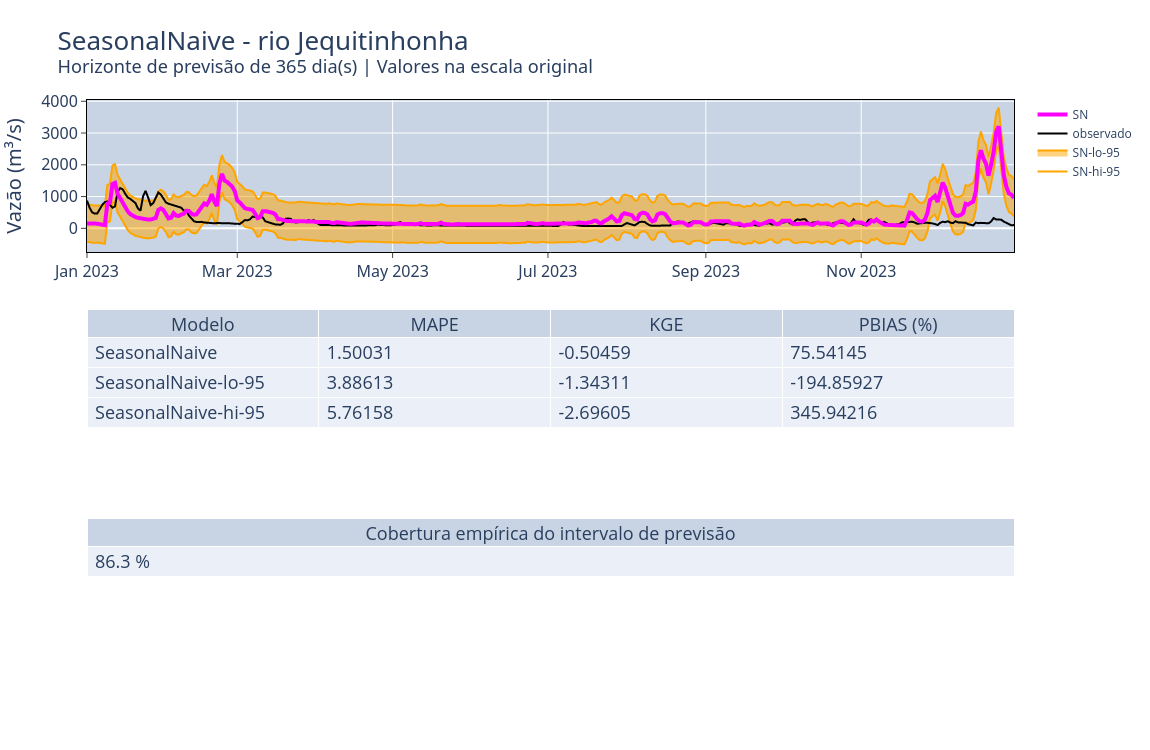
\includegraphics[scale=0.33]{Figuras/jequiti/wfv/SN/SN_WFV_ORIG.png}
	\caption{Resultado do SeasonalNaive no teste \textit{Walk-Forward Validation}\\(fonte: o autor)}
	\label{fig:jequiti_SN_WFV_ORIG}
\end{figure}

%\begin{table}[!h]
%	\centering \small
%	\caption{Resultados SeasonalNaive - rio Jequitinhonha \\(fonte: o autor)}
%	\begin{tabular}{|l|r|r|r|r|r|r|} \hline 
	%		\textbf{Horizonte} & \textbf{MAPE} & \textbf{RMSE} & \textbf{PBIAS} \\\hline
	%		1 dia              & 0,871         & 831,44        & -87,11 \\\hline
	%		3 dias             & 1,528         & 1872,25       & 102,71 \\\hline
	%		7 dias             & 1,046         & 1529,13       & 49,64  \\\hline
	%		15 dias            & 0,791         & 1468,02       & -13,46 \\\hline
	%	\end{tabular}
%	\label{tab:sn_jequitinhonha_resultados}
%\end{table}

Os resultados obtidos utilizando o modelo de Regressão Linear mostraram-se bastante promissores.(figura \ref{fig:jequiti_LR_WFV_LOG}) Nesta primeira avaliação, os dados foram log-transformados. Isso é verificável pelo título com o uso de ``destransformados''. Os dados foram log-transformados e retornados para a escala original para desenhar o gráfico e ficarem acessíveis para quem lê. \underline{Essa dinâmica no título se manterá por todo trabalho}.

Partindo pela KGE calculada, o resultado mostrou-se excelente. Recordando: quanto mais próxima de 1, melhor. Este valor sugere que o modelo é eficaz na previsão do comportamento hidrológico do sistema em análise, oferecendo previsões que estão bem alinhadas com os dados observados. A MAPE de $14,5\%$ sugere que o modelo tem uma precisão razoável e é bastante confiável. O modelo apresentou um viés sistemático de subestimar os resultados, conforme aponta a PBIAS de $-0,97\%$. Considerando todas as métricas, o resultado indica que o modelo teve um desempenho global muito bom. A KGE alta é particularmente indicativa de um bom ajuste global, com o modelo capturando bem tanto a dinâmica quanto a magnitude dos dados observados.

Considerando a qualidade dos intervalos de previsão, a cobertura observada de $98,08\%$ excedeu o intervalo teórico calculado de $95\%$, o que, à primeira vista, poderia ser interpretado como um desempenho satisfatório. No entanto, o limite superior do intervalo (hi-95) mostrou-se excessivamente elevado nos meses de janeiro e fevereiro, o que pode comprometer a interpretação dos resultados. Isso ocorre porque intervalos de previsão excessivamente amplos podem capturar praticamente qualquer valor observado, reduzindo a utilidade prática da previsão.

É importante destacar que os intervalos de previsão são calculados a partir dos erros do modelo durante a etapa de treinamento (\textit{in-sample residuals}). Para uma análise mais aprofundada desse comportamento, é necessário examinar os dados anteriores a 2023. A figura \ref{fig:jequiti_LR_final_2022_detalhe} revela que, nos últimos dias de 2022, houve observações significativamente elevadas. É provável que os erros associados a esse período mais próximo tenham influenciado a amplitude dos intervalos de previsão subsequentes. Essa interpretação é suportada pela observação de que o comportamento ao final de 2023 foi mais estável, possivelmente devido à ausência de eventos ruidosos imediatamente anteriores (meses de maio a agosto).

\begin{figure}[!h]
	\centering
	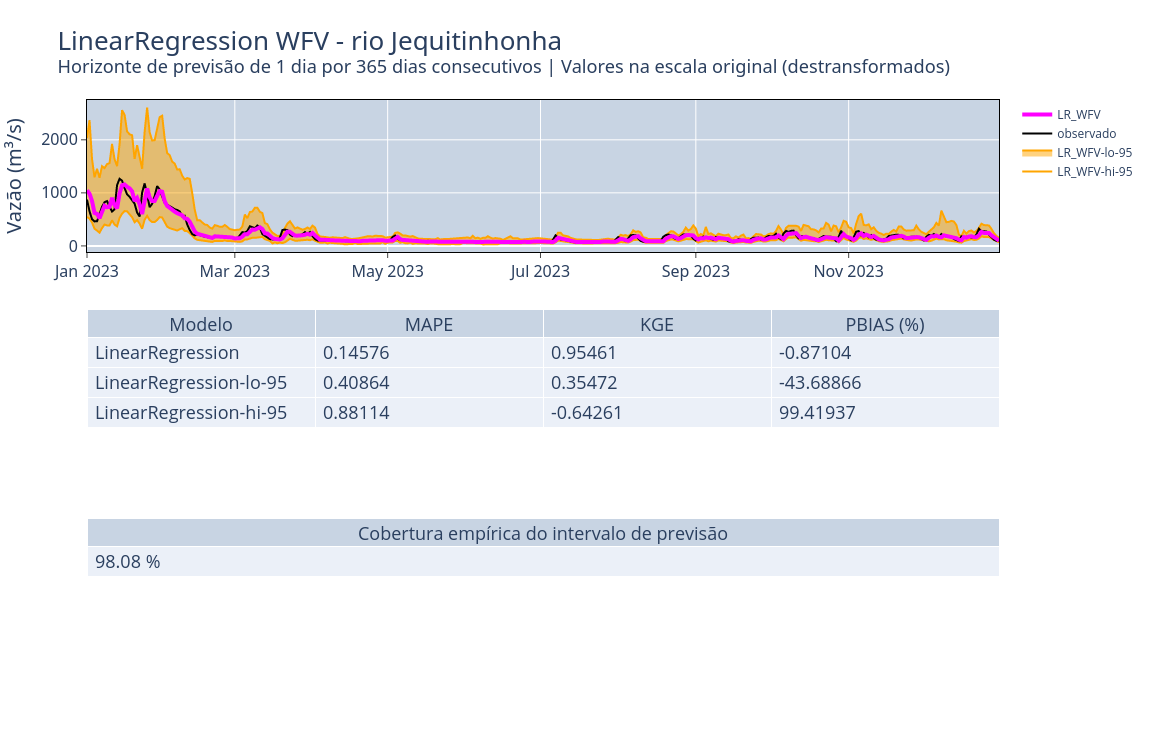
\includegraphics[scale=0.33]{Figuras/jequiti/wfv/LR/LR_WFV_LOG.png}
	\caption{\textit{Walk-Forward Validation} para o modelo Regressão Linear - LR\\(fonte: o autor)}
	\label{fig:jequiti_LR_WFV_LOG}
\end{figure}

\begin{figure}[!h]
	\centering
	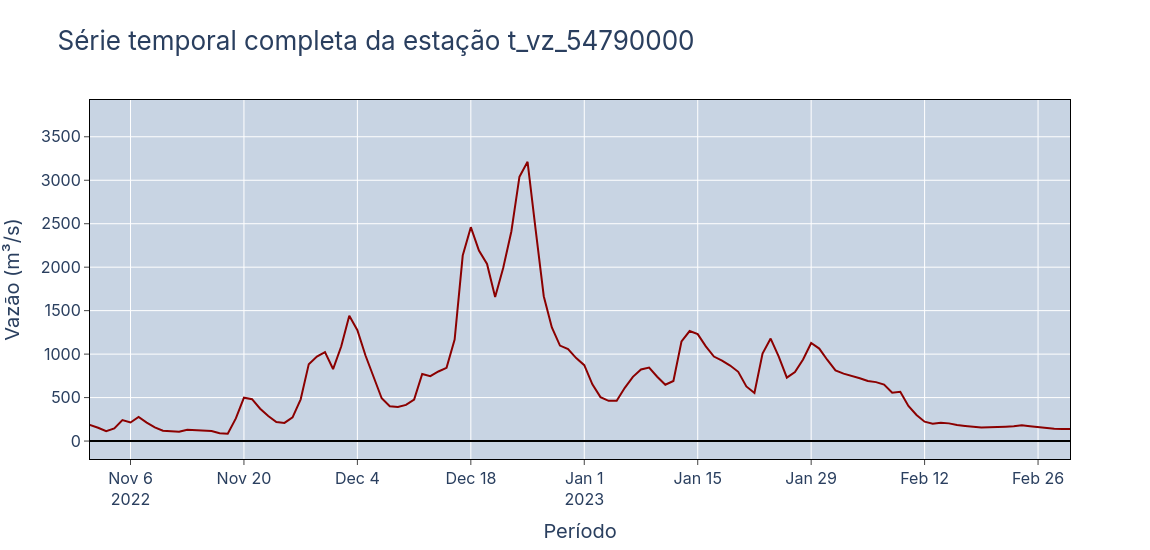
\includegraphics[scale=0.33]{Figuras/jequiti/LR_final_2022_detalhe.png}
	\caption{Detalhe do trecho final dos dados, em 2022, usados para treinamento.\\(fonte: o autor)}
	\label{fig:jequiti_LR_final_2022_detalhe}
\end{figure}

%A análise de \textit{delay} mostrou um resultado médio de $-0,87$. Se pegar a série prevista pelo modelo e comprimir linearmente em $-0,87$, ambas as sequências serão idênticas, ou seja, a série prevista será a série observada. Considerando que os dados estão numa frequência diária, isso pode ser interpretado como o modelo atrasando a previsão em $0,87$ dias, o que seria menos de 24 horas entre o evento ocorrer e ele ser percebido na previsão. Afirmar que o modelo está atrasado 20,88 horas, talvez, não convirja com a realidade, por isso que se considerar o desvio-padrão no resultado, confere mais coerência, pois indicaria que o atraso percebido no fenômeno é de cerca de um dia e meio, dois dias.

\begin{figure}[!h]
	\centering
	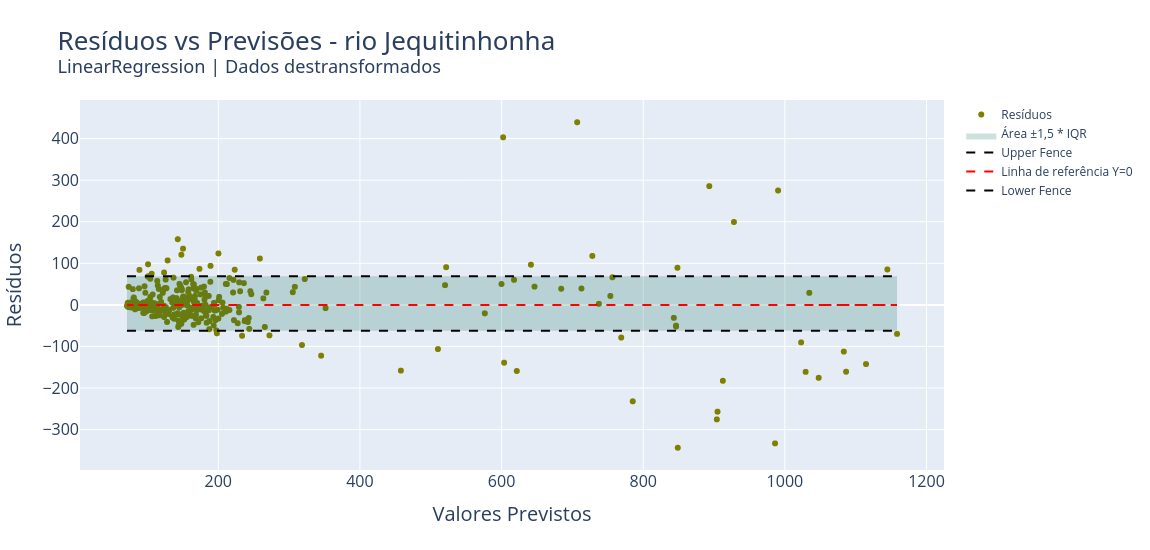
\includegraphics[scale=0.33]{Figuras/jequiti/wfv/LR/LR_WFV_LOG_RESID_x_PREV.png}
	\caption{Dispersão dos resíduos.\\(fonte: o autor)}
	\label{fig:jequiti_LR_WFV_LOG_RESID_x_PREV}
\end{figure}

Na figura \ref{fig:jequiti_LR_WFV_LOG_RESID_x_PREV} podemos observar a concentração dos resíduos em torno de zero. A linha vermelha tracejada é onde o valor previsto e observado são iguais, designando a previsão perfeita, com resíduo $0$. Este é o comportamento que se espera, idealmente, os resíduos estarem distribuídos aleatoriamente em torno de zero, sem padrões evidentes (nenhuma tendência clara de curvatura ou cone). Contudo, à medida que se caminha sobre a linha vermelha tracejada, aumentando o valor no eixo x, há um aumento na dispersão dos resíduos. A área sombreada demarcada são os valores calculados para \textit{lower fence} e \textit{upper fence} a partir do primeiro ($-12,83$) e terceiro ($19,98$) quartil, que aqui resultaram em $-62,06$ e $69,21$, respectivamente. Entre estes valores é onde se espera que os resíduos estejam distribuídos (houve uma prevalência de $87,4\%$ dos resíduos nesta área), o que fica de fora dessas faixas pode ser interpretado como um \textit{outlier}. Considerando que os dados de treinamento não foram tratados para valores \textit{outliers}, isso parece estar se refletindo neste resultado, mesmo com a transformação logarítmica. O modelo não captou corretamente os valores elevados nos dados observados, por isso resíduos tão grandes assim, ainda que tenha apresentado um comportamento geral bom, como visto nas métricas anteriormente. Outro fator a se considerar também é que por estar na escala log, qualquer pequena variação nesta escala, quando retornada para a escala original, pode significar números elevados.

Veja na figura \ref{fig:jequiti_LR_WFV_LOG_RESID_x_TEMPO} como os resíduos estão dispersos ao longo do tempo. No início do ano e final do ano, exatamente quando os eventos de chuva mais ocorrem, o modelo tende a se dispersar. No início do ano, como discutido anteriormente, pode ser que devido às vazões elevadas do final do ano de 2022, isso tenha causado ruídos em excesso na previsão do modelo. Quando houve vazões mais moderadas, os resíduos foram também mais moderados, como pode-se observar no final do ano de 2023, em que a influência imediata é o meio do ano, meses de inverno, e início de primavera. Quando da estação de baixa dos rios, os meses de outono e inverno, os resíduos estiveram bem alinhados em torno do $0$. Para encerrar essa análise, a figura \ref{fig:jequiti_LR_WFV_LOG_RESID_x_CURVA_NORMAL} apresenta que os resíduos estão próximos da normalidade quanto à distribuição destes em torno de $0$, com uma assimetria de $0,48$. O valor positivo para assimetria sugere que houve casos em que o modelo subestimou os valores (existe uma cauda à direita do centro dos dados), o que combina com os gráficos anteriores de dispersão. Mas cabe destacar que os resíduos não estão significativamente desviados em nenhuma direção, apresentam distribuição aleatória e não sistemática e este é um comportamento desejado. A análise da função de autocorrelação (ACF) está na figura \ref{fig:jequiti_LR_WFV_LOG_RESID_ACF} e aqui é analisado se existe independência ou dependência temporal entre os resíduos. A área sombreada representa a faixa ideal de permanência dos resíduos, onde se espera que a maioria dos resíduos esteja concentrada caso não haja autocorrelação significativa. Algumas \textit{lags} estão fora destes limites (picos), mais precisamente, \textit{lags} que estão mais próximas da \textit{lag} de referência. Este comportamento indica que o modelo pode ser refinado para melhor capturar dinâmicas temporais, possivelmente incorporando termos de tendência. Mas no aspecto geral, está bom o comportamento dos resíduos. Para melhorar os resíduos com valores tão elevados um tratamento de \textit{outliers} pode verter bons resultados.

\begin{figure}[!h]
	\centering
	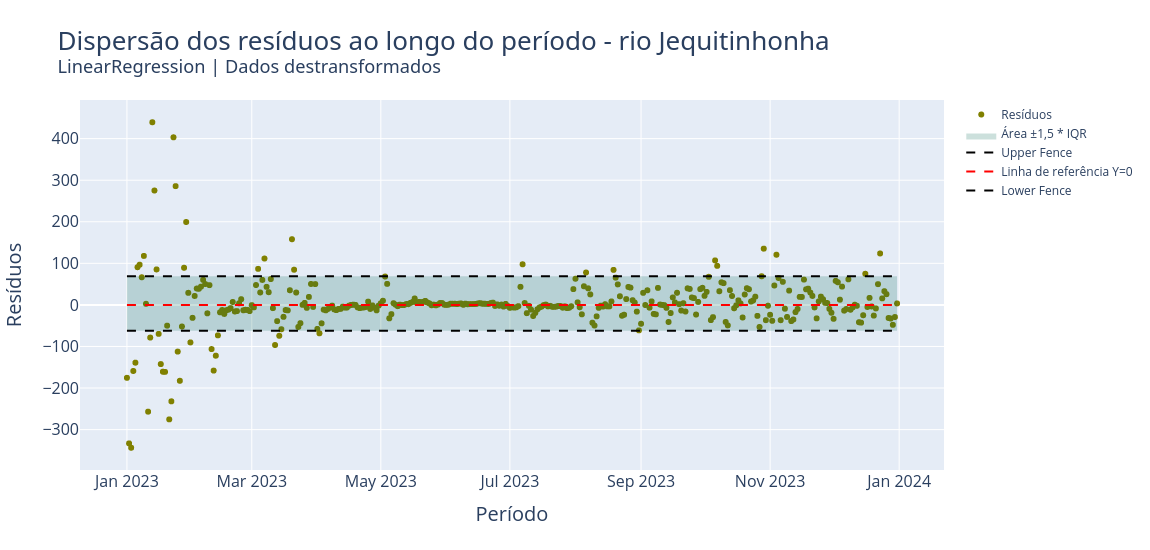
\includegraphics[scale=0.33]{Figuras/jequiti/wfv/LR/LR_WFV_LOG_RESID_x_TEMPO.png}
	\caption{Resíduos da previsão ao longo do tempo.\\(fonte: o autor)}
	\label{fig:jequiti_LR_WFV_LOG_RESID_x_TEMPO}
\end{figure}

\begin{figure}[!h]
	\centering
	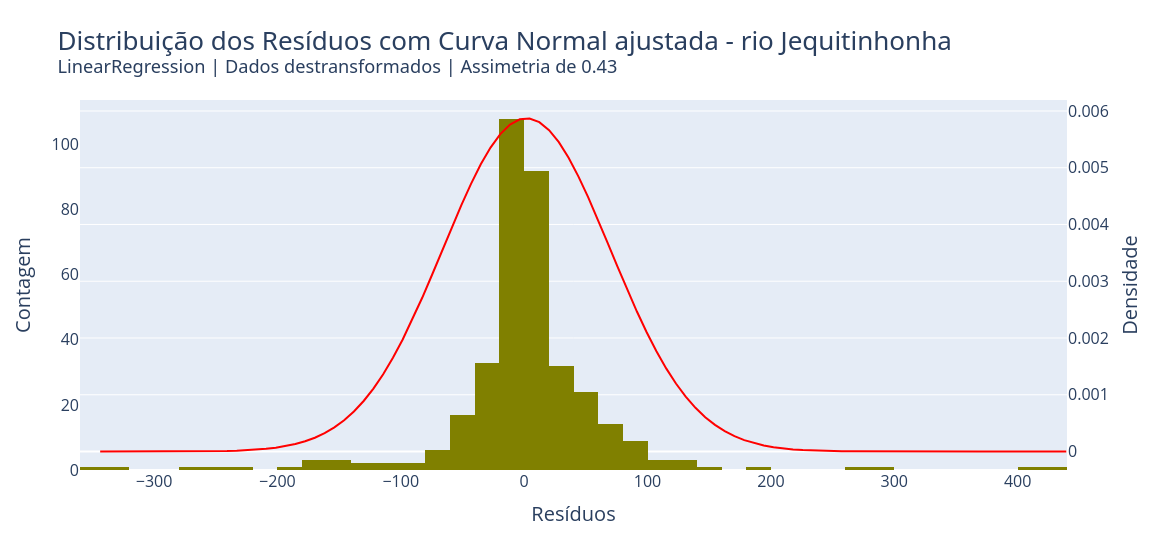
\includegraphics[scale=0.33]{Figuras/jequiti/wfv/LR/LR_WFV_LOG_RESID_x_CURVA_NORMAL.png}
	\caption{Histograma dos resíduos.\\(fonte: o autor)}
	\label{fig:jequiti_LR_WFV_LOG_RESID_x_CURVA_NORMAL}
\end{figure}

\begin{figure}[!h]
	\centering
	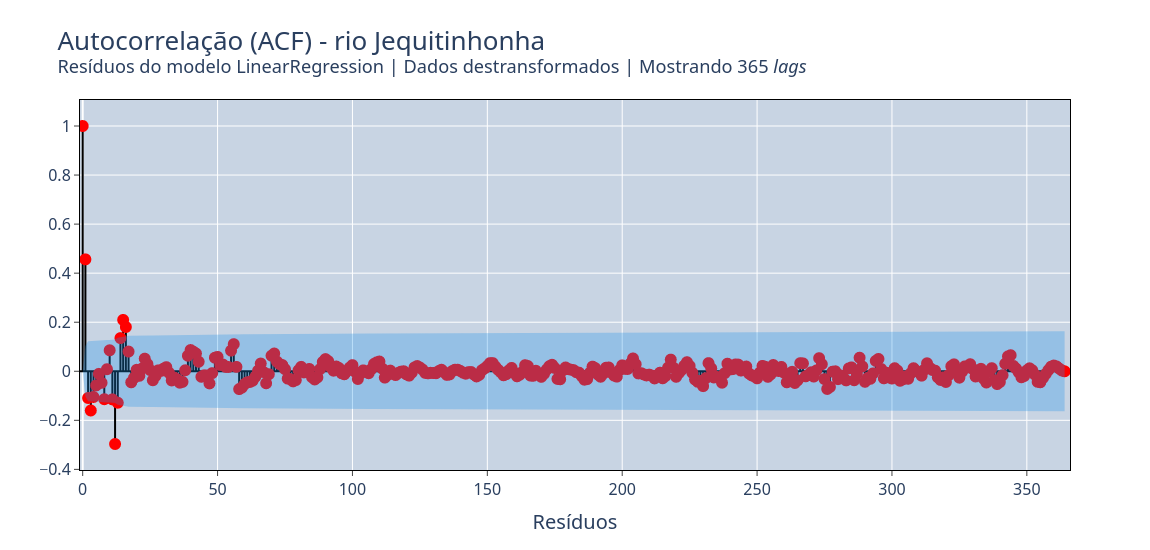
\includegraphics[scale=0.33]{Figuras/jequiti/wfv/LR/LR_WFV_LOG_RESID_ACF.png}
	\caption{Resíduos da previsão ao longo do tempo.\\(fonte: o autor)}
	\label{fig:jequiti_LR_WFV_LOG_RESID_ACF}
\end{figure}
\clearpage

Agora os resultados sem emprego da log-transformação, com os dados originais. Salientando que para o modelo LR não é correto aplicar os dados originais na escala em que se encontram, foi precisar realizar normalização antes empregando algoritmo MinMax. Este algoritmo coloca todos os dados em valores entre $0$ e $1$, sendo o valor mínimo correspondente a cada série temporal passado para $0$ e o valor máximo é passado para $1$. Com os demais valores é feito, basicamente, uma regra de três para achar o valor correspondente na escala entre $0$ e $1$.

Dito isso, o resultado para os dados originais ficou levemente inferior ao modelo com os dados log-transformados. Em todas as métricas que se avaliar o resultado ficou piorado. Um comportamento destacado foi as faixas nos valores dos intervalos de previsão. Diferentemente do comportamento anterior (figura \ref{fig:jequiti_LR_WFV_LOG}), em que houve uma prevalência de faixas elevadas no início do ano, neste resultado o início do ano esteve, digamos, bem comportado. Ao decorrer do ano que os intervalos incrementaram, ali a partir do mês de fevereiro, e foram aumentando até o fim do ano. Isso pode ser um indicativo de que o modelo teve problemas na estabilidade de longo prazo, acumulando incertezas no período.

Ainda que tenha apresentado uma KGE inferior, bem como nas demais métricas, quando se observa o comportamento dos resíduos, houve uma prevalência de $91,78\%$ dos resíduos na área sombreada no gráfico de dispersão.(figura \ref{fig:jequiti_LR_WFV_SCLD_RESID_x_PREV}) Isso significa que houve menos \textit{outliers} nas previsões. Pode-se verificar também este resultado na figura \ref{fig:jequiti_LR_WFV_SCLD_RESID_x_TEMPO}, no início do ano, em que menos \textit{outliers} estão presentes, ainda que na porção final do ano tenha aparecido alguns a mais que não foram vistos na análise anterior (figura \ref{fig:jequiti_LR_WFV_LOG_RESID_x_TEMPO}). Para os dados originais, ainda que nas métricas pareça piorado, pela análise dos resíduos o modelo mostrou boa estabilidade nas previsões pontuais. Quando se considera os intervalos de previsão, precisa considerar com parcimônia, visto que o crescimento dos valores superioes (hi-95) e valores de vazão $0 m^3/s$ na faixa inferior (lo-95) indicam instabilidade de longo prazo.

%Para a análise de \textit{delay}, o mesmo feito anteriormente serve para este: aplicar o valor do desvio-padrão parece ser mais coerente com o comportamento real, sendo que aqui houve uma piora significativa no atraso, passando para mais de 3 dias ($3,78$).

Caminhando para o fim, o histograma e curva-normal apresentou uma assimetria consideravelmente superior ($3,37$) ao resultado de antes, com presença de cauda longa à direita.(figura \ref{fig:jequiti_LR_WFV_SCLD_RESID_x_CURVA_NORMAL}) O modelo teve tendência de subestimar os resultados, o que é verificável pelo PBIAS. Na figura \ref{fig:jequiti_LR_WFV_SCLD_RESID_ACF} é possível perceber picos fora do intervalo de confiança. Depois de cerca de 10 lags, os pontos de autocorrelação ficam dentro desta faixa, indicando que a maioria dos resíduos após esse ponto não está significativamente correlacionada com valores anteriores. Este pontos vermelhos no início do gráfico indicam que pode haver correlações significativas entre os resíduos com pequenos \textit{lags}, o que sugere, nos primeiros períodos, que os resíduos estão correlacionados com os valores anteriores. Isso é indicativo de que o modelo pode não estar capturando totalmente a estrutura temporal dos dados. Pode ser necessário ajustar o modelo, adicionar variáveis que expliquem essa dependência temporal, ainda que variáveis de valor acumulado tenham sido inseridas exatamente na intenção de capturar tais comportamentos. Mas claramente precisaria aprimorar.

\begin{figure}[!h]
\centering
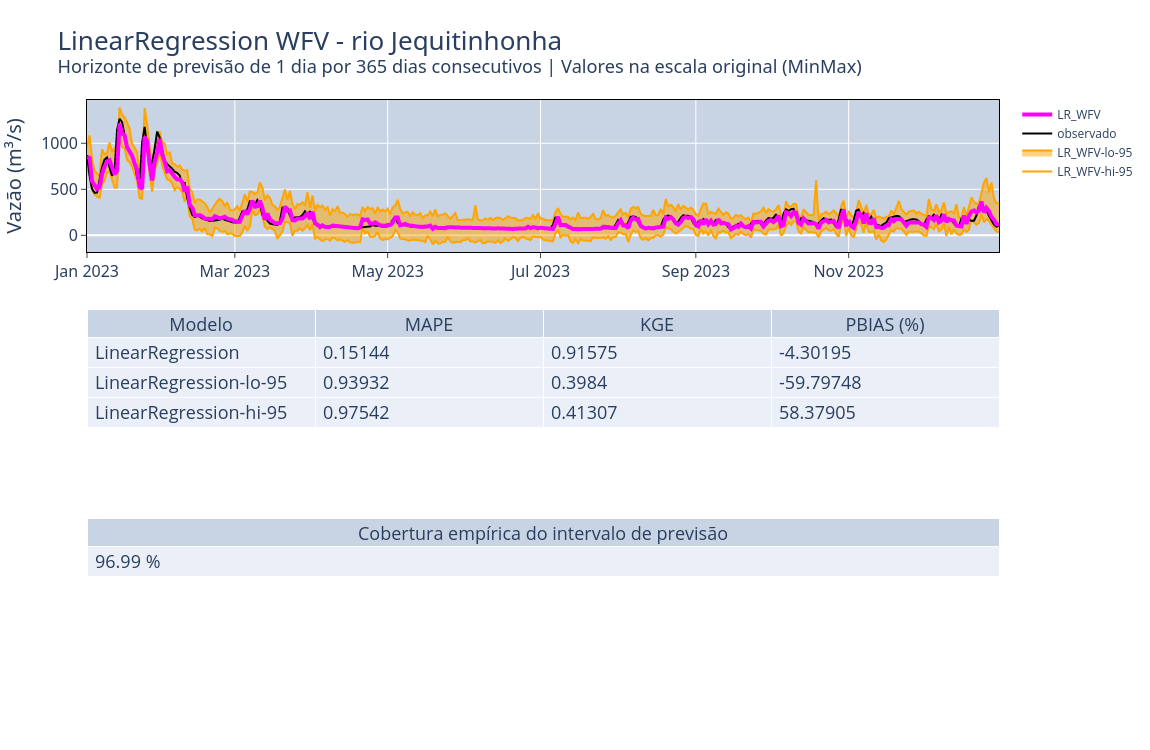
\includegraphics[scale=0.33]{Figuras/jequiti/wfv/LR/LR_WFV_ORIG.png}
\caption{\textit{Walk-Forward Validation} para o modelo Regressão Linear - LR.\\(fonte: o autor)}
\label{fig:jequiti_LR_WFV_ORIG}
\end{figure}

\begin{figure}[!h]
\centering
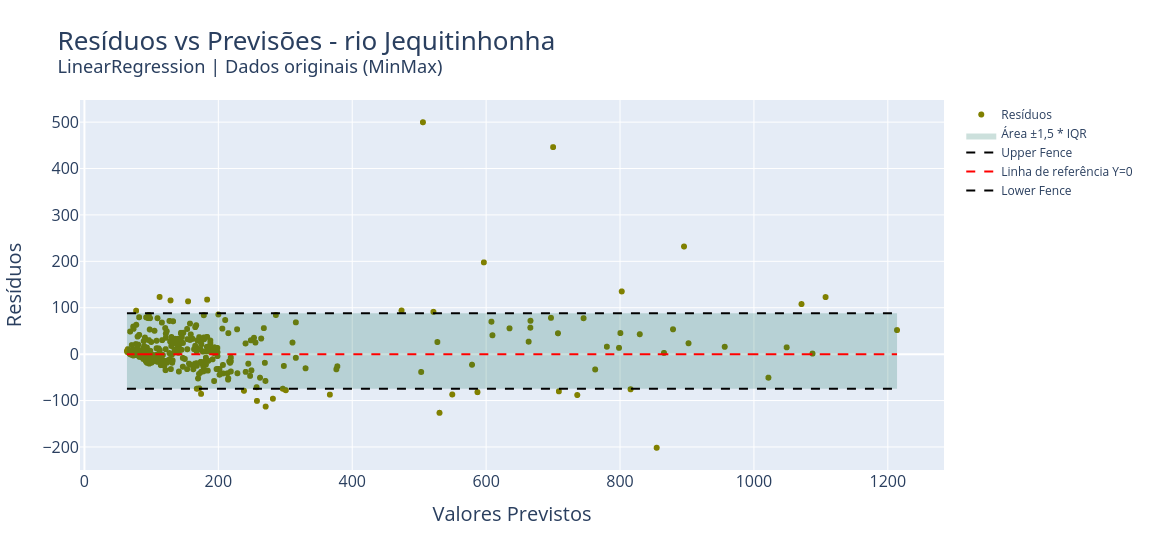
\includegraphics[scale=0.33]{Figuras/jequiti/wfv/LR/LR_WFV_ORIG_RESID_x_PREV.png}
\caption{Dispersão dos resíduos.\\(fonte: o autor)}
\label{fig:jequiti_LR_WFV_ORIG_RESID_x_PREV}
\end{figure}

\begin{figure}[!h]
\centering
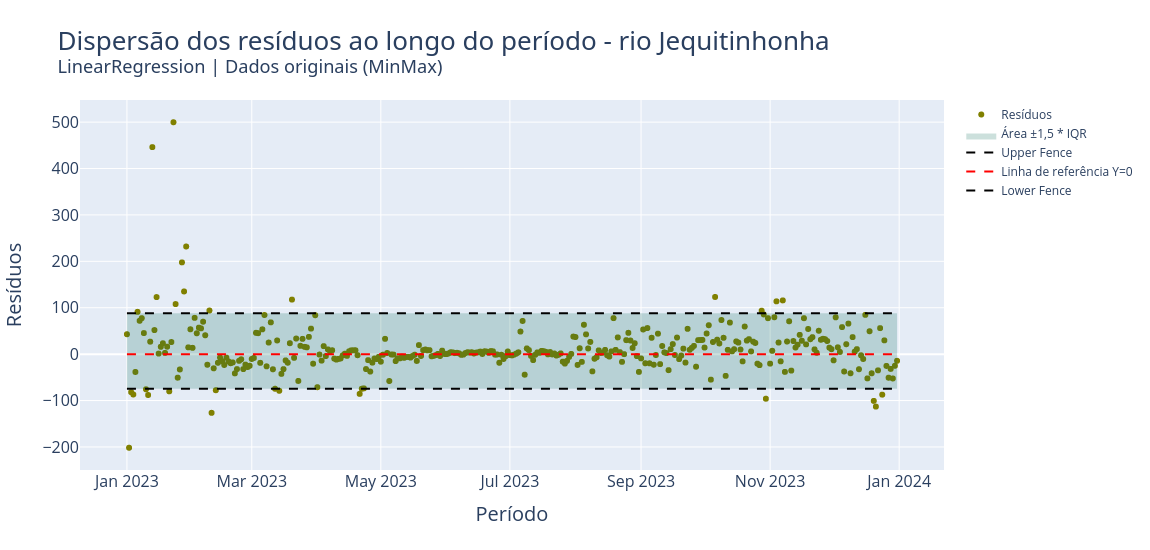
\includegraphics[scale=0.33]{Figuras/jequiti/wfv/LR/LR_WFV_ORIG_RESID_x_TEMPO.png}
\caption{Dispersão dos resíduos ao longo do ano.\\(fonte: o autor)}
\label{fig:jequiti_LR_WFV_ORIG_RESID_x_TEMPO}
\end{figure}

\begin{figure}[!h]
\centering
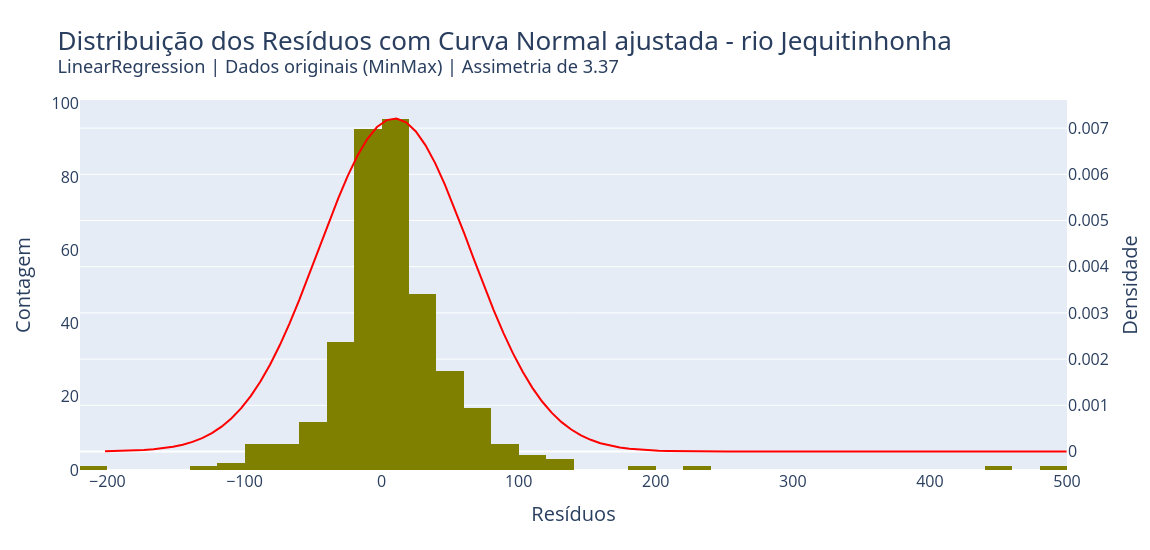
\includegraphics[scale=0.33]{Figuras/jequiti/wfv/LR/LR_WFV_ORIG_RESID_x_CURVA_NORMAL.png}
\caption{Histograma e curva-normal dos resíduos.\\(fonte: o autor)}
\label{fig:jequiti_LR_WFV_ORIG_RESID_x_CURVA_NORMAL}
\end{figure}

\begin{figure}[!h]
\centering
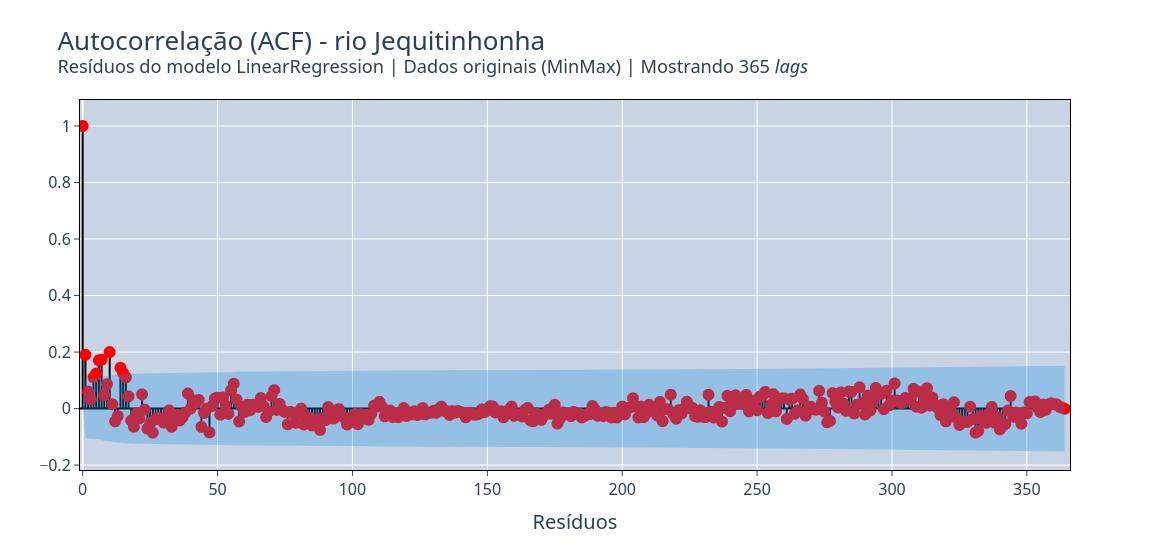
\includegraphics[scale=0.33]{Figuras/jequiti/wfv/LR/LR_WFV_ORIG_RESID_ACF.png}
\caption{Gráfico ACF dos resíduos.\\(fonte: o autor)}
\label{fig:jequiti_LR_WFV_ORIG_RESID_ACF}
\end{figure}
\clearpage

Passando agora à análise dos modelos principais deste trabalho, cujos resultados serão comparados ao modelo de referência, optou-se por realizar a análise de forma concomitante, uma vez que ambos os modelos apresentaram comportamentos similares, embora o modelo RandomForest tenha demonstrado um desempenho superior ao CatBoost.

Na métrica KGE, comparando-se os resultados com o comportamento ilustrado na figura \ref{fig:jequiti_LR_WFV_LOG}, observa-se que ambos os modelos não conseguiram superar o modelo de referência, com destaque para o CB, que apresentou uma performance consideravelmente inferior. No entanto, ao considerar a precisão percentual média, avaliada pela métrica MAPE, ambos os modelos baseados em árvores apresentaram melhorias em relação ao modelo de referência, evidenciando um desempenho superior em termos de erro percentual médio.

A KGE, relembrando, combina três aspectos fundamentais: variabilidade, viés e correlação entre os dados observados e previstos. Considerando esses fatores, com os dados log-transformados, o modelo LR capturou de forma mais eficaz os três aspectos mencionados. É provável que a linearização tenha sido um fator determinante para o bom desempenho deste modelo olhando por esta métrica, uma vez que, ao analisar a MAPE, os modelos não-lineares (CB e RF) apresentaram desempenhos melhores. Um desempenho médio percentual melhor pode dever-se à resiliência dos modelos não-lineares à sua robustez diante de valores discrepantes, aos quais o modelo linear é mais sensível.

Observa-se que tanto o CB quanto o RF apresentaram intervalos de previsão menos amplos no início do ano, em comparação com o modelo LR, mesmo impactados pelas vazões elevadas no final de 2022 (figura \ref{fig:jequiti_LR_final_2022_detalhe}). Em termos de previsão pontual, ambos os modelos não lineares demonstraram-se robustos. No entanto, ao analisar a cobertura empírica dos intervalos de previsão, o modelo RF mostrou-se consideravelmente defasado em relação aos modelos LR e CB. Isso pode ser explicado pela possível ``otimização'' excessiva do modelo ao calcular os intervalos, ao presumir uma repetição dos eventos e erros passados, resultando em intervalos estreitos. Esse fenômeno é descrito por \citet{RobHyndman_prediction_intervals}. Apesar disso, a cobertura empírica de $80\%$ do modelo RF ainda pode ser considerada satisfatória, e a cobertura de $88\%$ obtida pelo CB demonstra um bom desempenho.

Pode-se inferir que os modelos CB e RF conseguiram equilibrar a previsão pontual, indicada pela MAPE de $0,12$, com os intervalos de previsão. Um ajuste de hiperparâmetros poderia potencialmente melhorar esse desempenho. Em relação ao PBIAS, ambos os modelos apresentaram um desvio sistemático, subestimando os valores previstos.

%No que diz respeito ao \textit{delay}, todos os modelos, incluindo o LR, apresentaram um comportamento semelhante, com um atraso de aproximadamente 1 a 2 dias para que um evento na série observada fosse captado nas previsões. Essa análise leva em consideração o desvio-padrão.

\begin{figure}[!h]
\centering
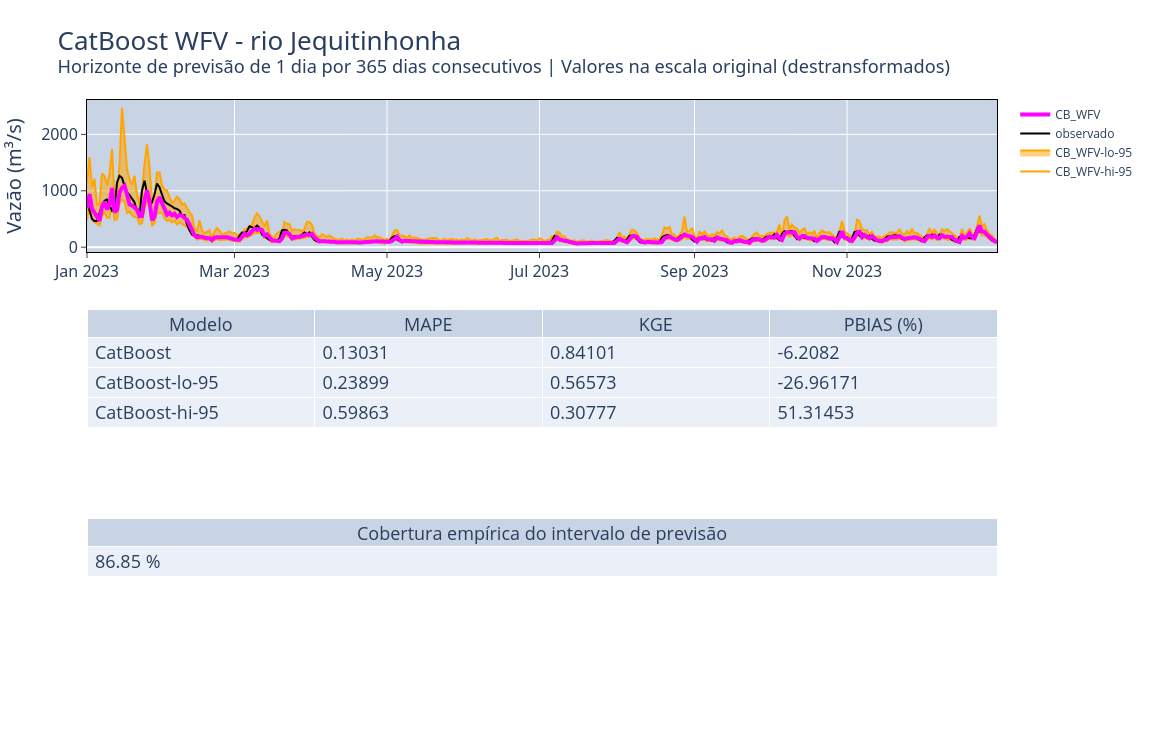
\includegraphics[scale=0.33]{Figuras/jequiti/wfv/CB/CB_WFV_LOG.png}
\caption{\textit{Walk-Forward Validation} para o modelo CatBoost - CB.\\(fonte: o autor)}
\label{fig:jequiti_CB_WFV_LOG}
\end{figure}

\begin{figure}[!h]
\centering
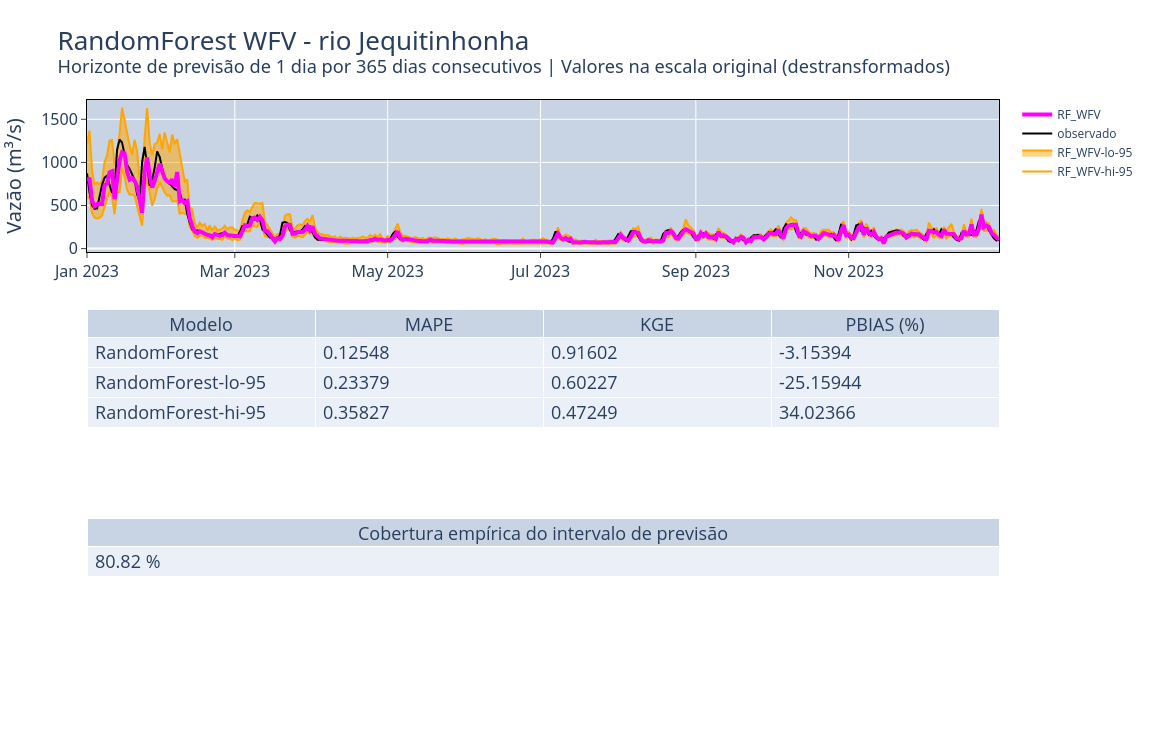
\includegraphics[scale=0.33]{Figuras/jequiti/wfv/RF/RF_WFV_LOG.png}
\caption{\textit{Walk-Forward Validation} para o modelo RandomForest - RF.\\(fonte: o autor)}
\label{fig:jequiti_RF_WFV_LOG}
\end{figure}
\clearpage

Os resíduos em modelos não-lineares podem ser mais difíceis de interpretar porque esses modelos capturam interações e padrões complexos. Porém, mesmo assim, detectar padrões sistemáticos nos resíduos ajuda a elucidar se os modelos conseguiram capturar todas as nuances dos dados.

Em ambos os casos, não houve prevalência de comportamento anormal para os resíduos. Estiveram aleatoriamente distribuídos em torno de $0$, com uma menção importante para a maior dispersão de possíveis valores \textit{outliers} para o modelo CB à medida que as medições aumentaram.(figura \ref{fig:jequiti_CB_WFV_LOG_RESID_x_PREV}).

\begin{figure}[!h]
\centering
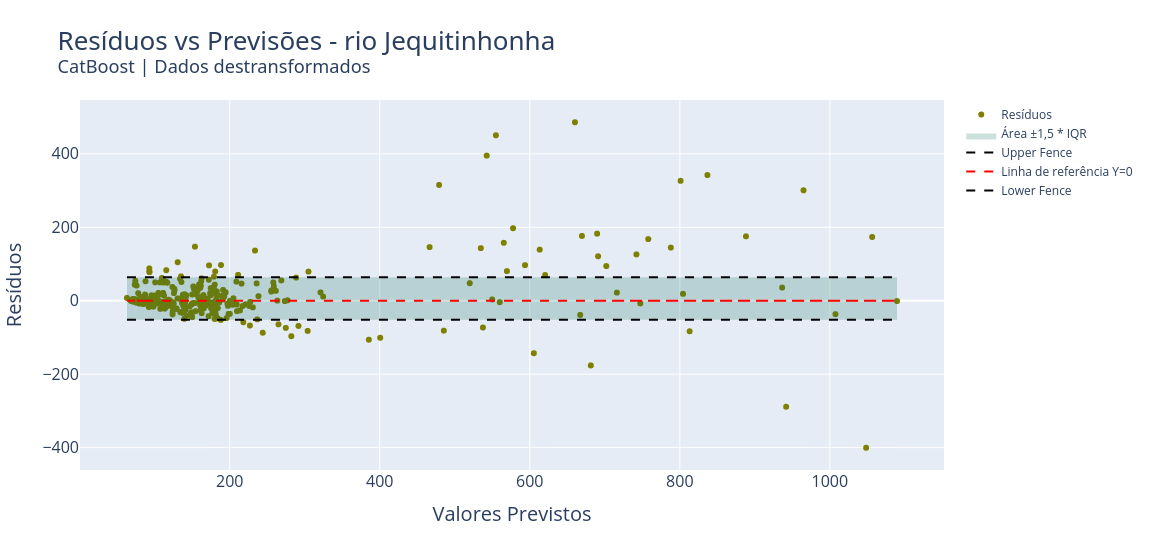
\includegraphics[scale=0.33]{Figuras/jequiti/wfv/CB/CB_WFV_LOG_RESID_x_PREV.png}
\caption{Dispersão dos resíduos.\\(fonte: o autor)}
\label{fig:jequiti_CB_WFV_LOG_RESID_x_PREV}
\end{figure}

\begin{figure}[!h]
\centering
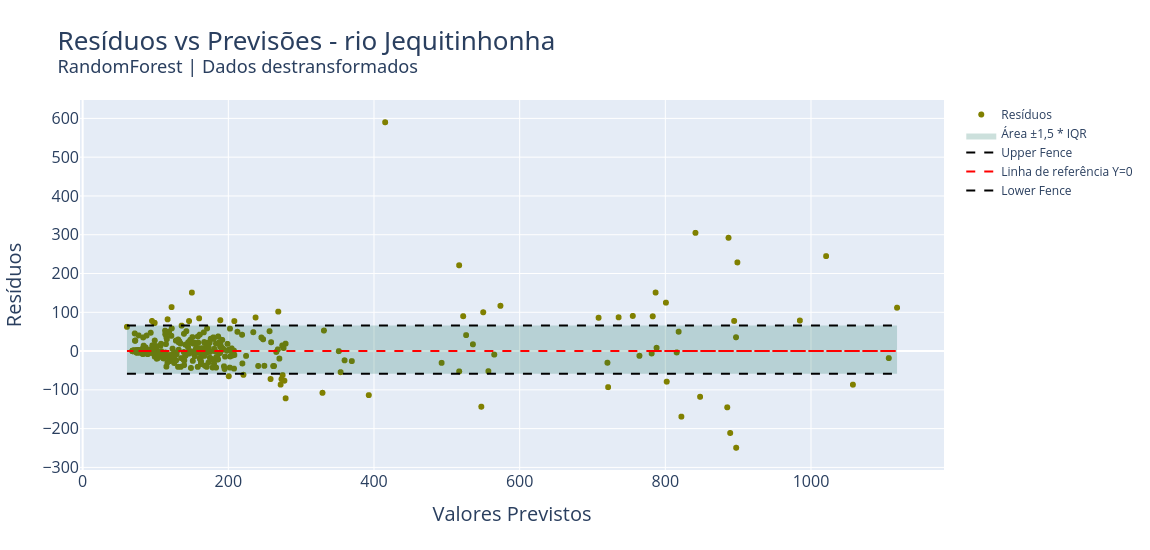
\includegraphics[scale=0.33]{Figuras/jequiti/wfv/RF/RF_WFV_LOG_RESID_x_PREV.png}
\caption{Dispersão dos resíduos.\\(fonte: o autor)}
\label{fig:jequiti_RF_WFV_LOG_RESID_x_PREV}
\end{figure}
\clearpage

A dispersão ao longo do tempo foi praticamente a mesma para ambos os modelos, com resíduos de valor elevado mais presentes no início da série. (figuras \ref{fig:jequiti_CB_WFV_LOG_RESID_x_TEMPO} \ref{fig:jequiti_RF_WFV_LOG_RESID_x_TEMPO}) Aqui vale a interpretação usada para o modelo de referência, de que os valores elevados aferidos em final de 2022 possam ter interferido. Houve uma prevalência de $84,11\%$ e $86,03\%$, respectivamente CB e RF, dos resíduos na área sombreada, correspondente à área de erro aceitável. Uma leve melhor prevalência para o modelo RF, que pode ser vista também em menos dispersão de resíduos para fora dos limites da área sombreada no início do ano.

\begin{figure}[!h]
\centering
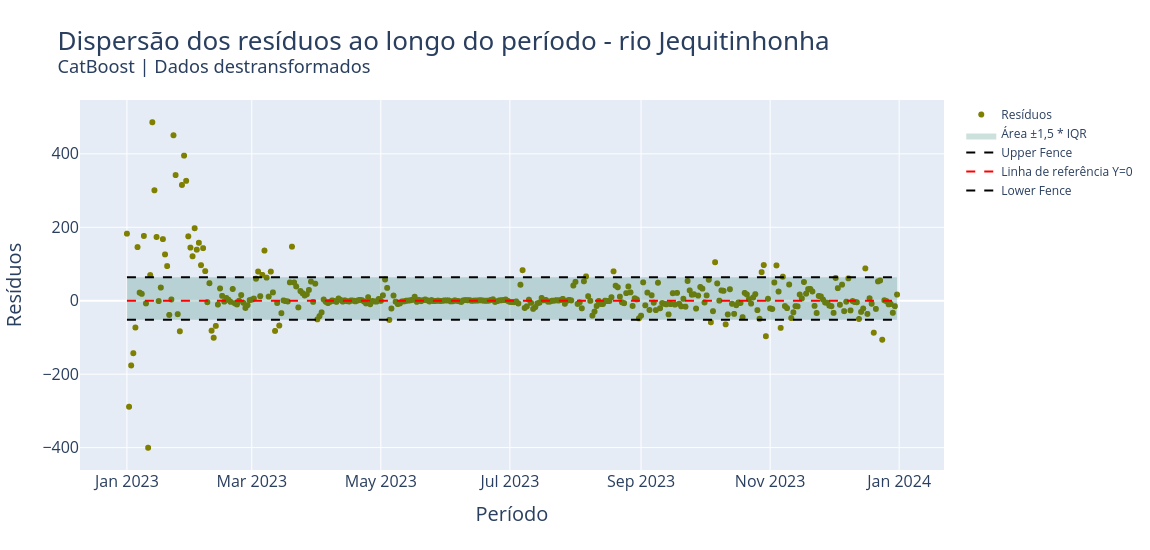
\includegraphics[scale=0.33]{Figuras/jequiti/wfv/CB/CB_WFV_LOG_RESID_x_TEMPO.png}
\caption{Dispersão dos resíduos ao longo do ano.\\(fonte: o autor)}
\label{fig:jequiti_CB_WFV_LOG_RESID_x_TEMPO}
\end{figure}

\begin{figure}[!h]
\centering
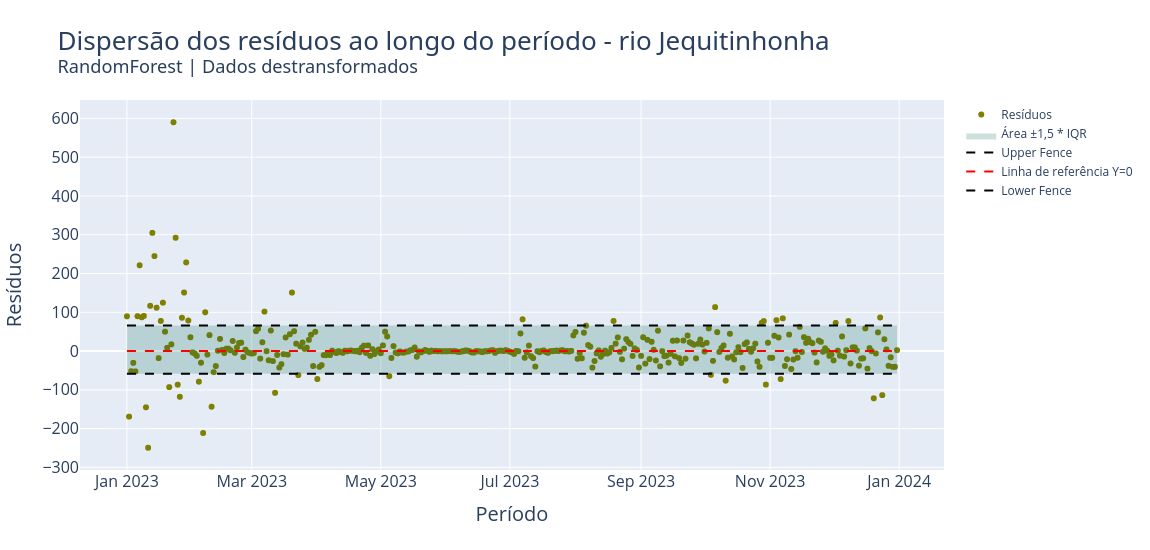
\includegraphics[scale=0.33]{Figuras/jequiti/wfv/RF/RF_WFV_LOG_RESID_x_TEMPO.png}
\caption{Dispersão dos resíduos ao longo do ano.\\(fonte: o autor)}
\label{fig:jequiti_RF_WFV_LOG_RESID_x_TEMPO}
\end{figure}
\clearpage

Em termos de assimetria da distribuição dos resíduos, ambos modelos comportaram-se iguais, com assimetria positiva indicando cauda à direita. Com valores de $2,56$ para o modelo CB e $2,54$ para o RF, isso mostra tendência de subestimar as previsões (visto no PBIAS de ambos os modelos).

\begin{figure}[!h]
\centering
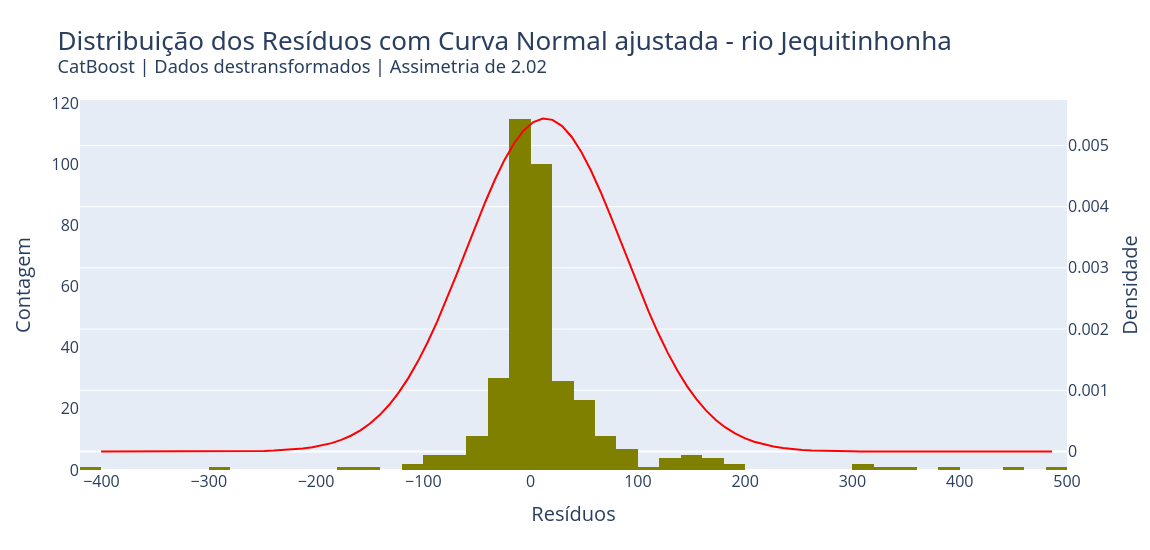
\includegraphics[scale=0.33]{Figuras/jequiti/wfv/CB/CB_WFV_LOG_RESID_x_CURVA_NORMAL.png}
\caption{Histograma e curva-normal dos resíduos.\\(fonte: o autor)}
\label{fig:jequiti_CB_WFV_LOG_RESID_x_CURVA_NORMAL}
\end{figure}

\begin{figure}[!h]
\centering
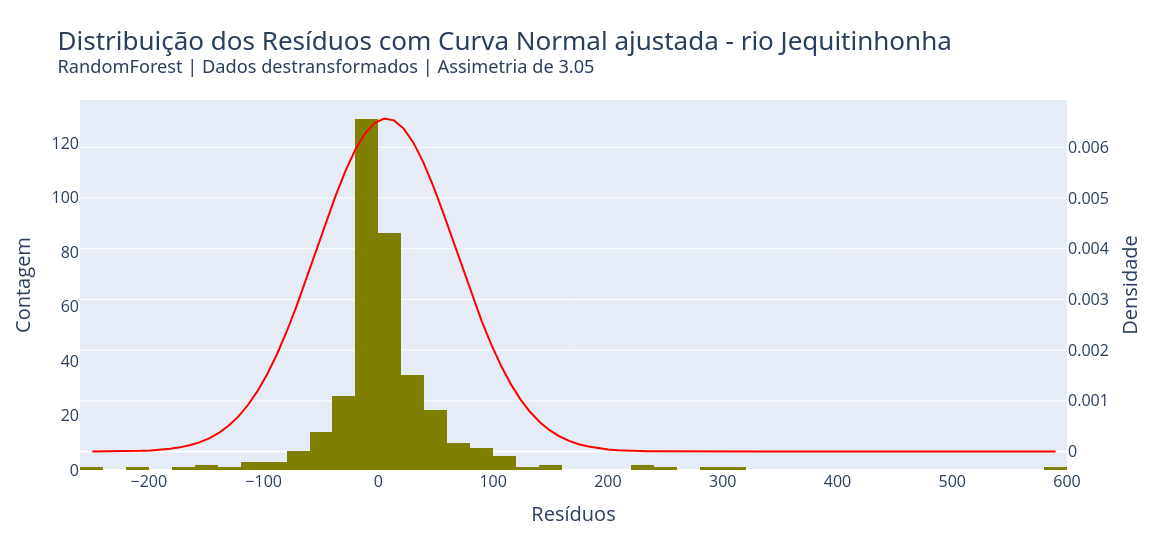
\includegraphics[scale=0.33]{Figuras/jequiti/wfv/RF/RF_WFV_LOG_RESID_x_CURVA_NORMAL.png}
\caption{Histograma e curva-normal dos resíduos.\\(fonte: o autor)}
\label{fig:jequiti_RF_WFV_LOG_RESID_x_CURVA_NORMAL}
\end{figure}
\clearpage

Observando os gráficos de autocorrelação dos modelos, houve um comportamento parecido nas \textit{lags} iniciais. Nas primeiras \textit{lags}, os gráficos mostram pontos de autocorrelação que ultrapassam a faixa de confiança (sombreada em azul), indicando que os resíduos possuem dependência temporal significativa nos primeiros períodos. Esse padrão sugere que os modelos não conseguiram capturar totalmente a estrutura temporal dos dados, resultando em resíduos correlacionados em curtos períodos de tempo. Uma possível explicação pode ser a presença de componentes sazonais ou padrões de curto prazo que não foram completamente modelados.

A partir de aproximadamente a \textit{lag} 20, a autocorrelação dos resíduos cai para valores próximos de zero e permanece dentro da faixa de confiança para as \textit{lags} seguintes até a \textit{lag} 365. Este é um comportamento esperado para um bom modelo, onde os resíduos devem ser independentes e distribuídos aleatoriamente ao longo do tempo. A presença de resíduos com baixa autocorrelação em \textit{lags} maiores indica que, em períodos mais longos, os modelos não apresentam problemas de dependência temporal.

\begin{figure}[!h]
\centering
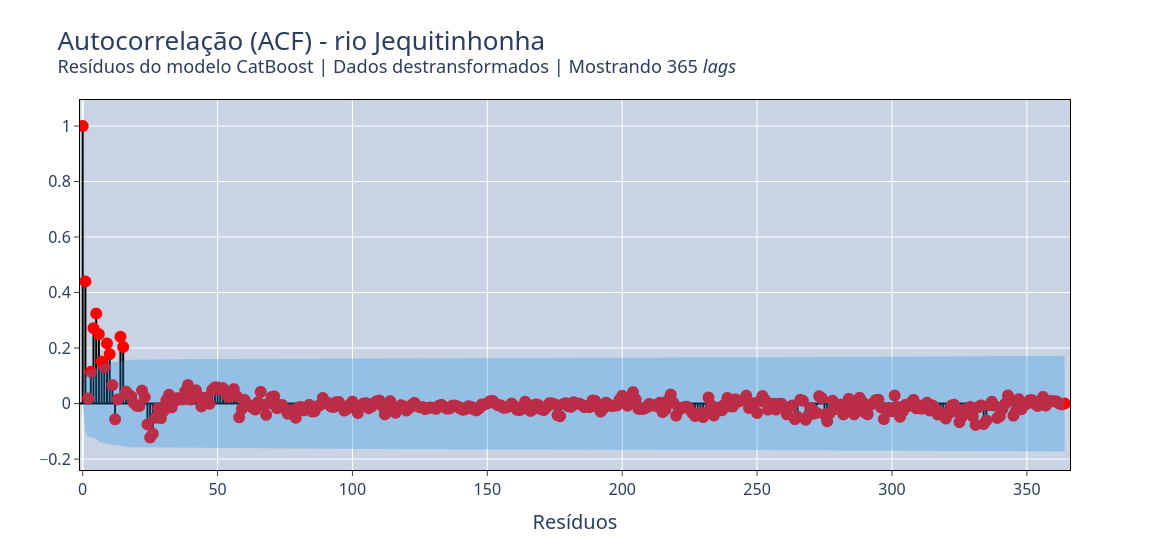
\includegraphics[scale=0.33]{Figuras/jequiti/wfv/CB/CB_WFV_LOG_RESID_ACF.png}
\caption{Gráfico ACF dos resíduos.\\(fonte: o autor)}
\label{fig:jequiti_CB_WFV_LOG_RESID_ACF}
\end{figure}

\begin{figure}[!h]
\centering
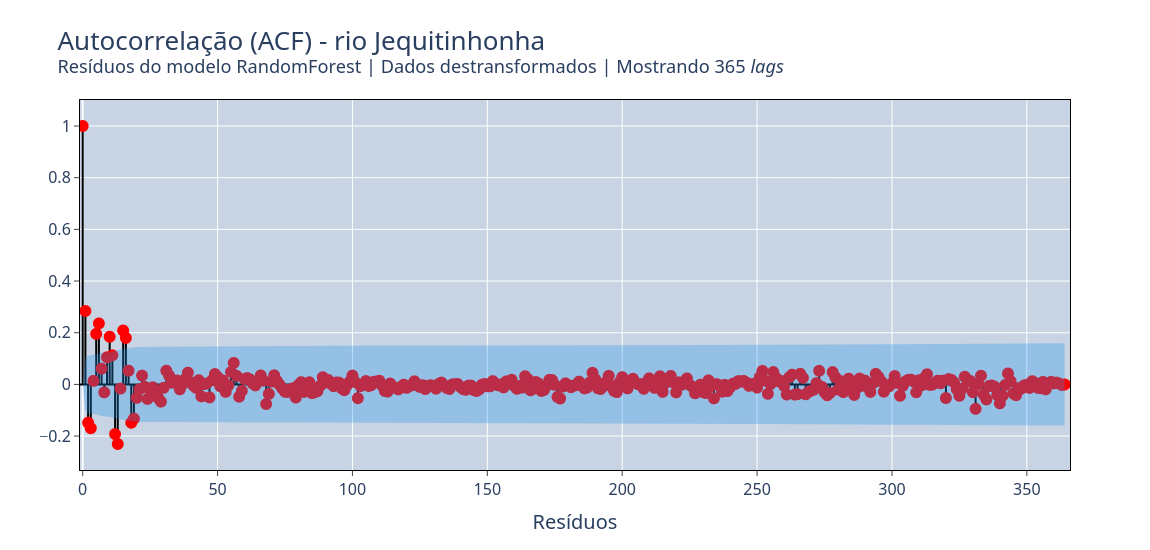
\includegraphics[scale=0.33]{Figuras/jequiti/wfv/RF/RF_WFV_LOG_RESID_ACF.png}
\caption{Gráfico ACF dos resíduos.\\(fonte: o autor)}
\label{fig:jequiti_RF_WFV_LOG_RESID_ACF}
\end{figure}
\clearpage

Neste momento será apresentado o resultado dos modelos CB e RF para os dados em sua escala original, sem a log-transformação. Recapitulando: a log-transformação lineariza os dados e para o modelo LR ela realmente resultou em melhora do comportamento do modelo. Esperava-se que o mesmo pudesse, eventualmente, ocorrer com estes modelos não-lineares, pois simplificaria as relações entre as variáveis. Porém, aconteceu o oposto. Permanecer com os dados originais, \textit{in natura} por assim dizer, foi o que fez ambos se comportarem melhor.

Veja o comportamento do \textit{walk-forward validation}. Houve melhoras em todas métricas nos dois modelos, com exceção para o modelo RF, que a MAPE piorou com os dados originais em relação aos dados log-transformados, ficando $1,4\%$ acima. É ínfimo, porém não descartável. Mas a KGE, uma métrica mais robusta, melhorou bastante entre o resultado anterior e este resultado em tela. Aplicando os modelos CB e RF nos dados originais, melhorou também o viés sistemático (PBIAS). O modelo CB continuou mostrando tendência de subestimar as previsões mas aqui o modelo RF inverteu, passando a apresentar tendência de superestimar as previsões. A cobertura empírica dos intervalos de previsão melhoraram, sendo o CB pouco mais de $1\%$ melhor, mas o RF melhorou mais de $4\%$ nos cálculos dos intervalos. À respeito dos intervalos de previsão, os modelos mostraram tendência de aumento das faixas ao longo do ano. Diferentemente da análise log-transformada, aqui os modelos parecem ter demostrado incerteza quanto aos erros calculados em eventos anteriores, ainda que no início do ano, para ambos, pareça ter ficado mais estável o cálculo dos intervalos.

\begin{figure}[!h]
\centering
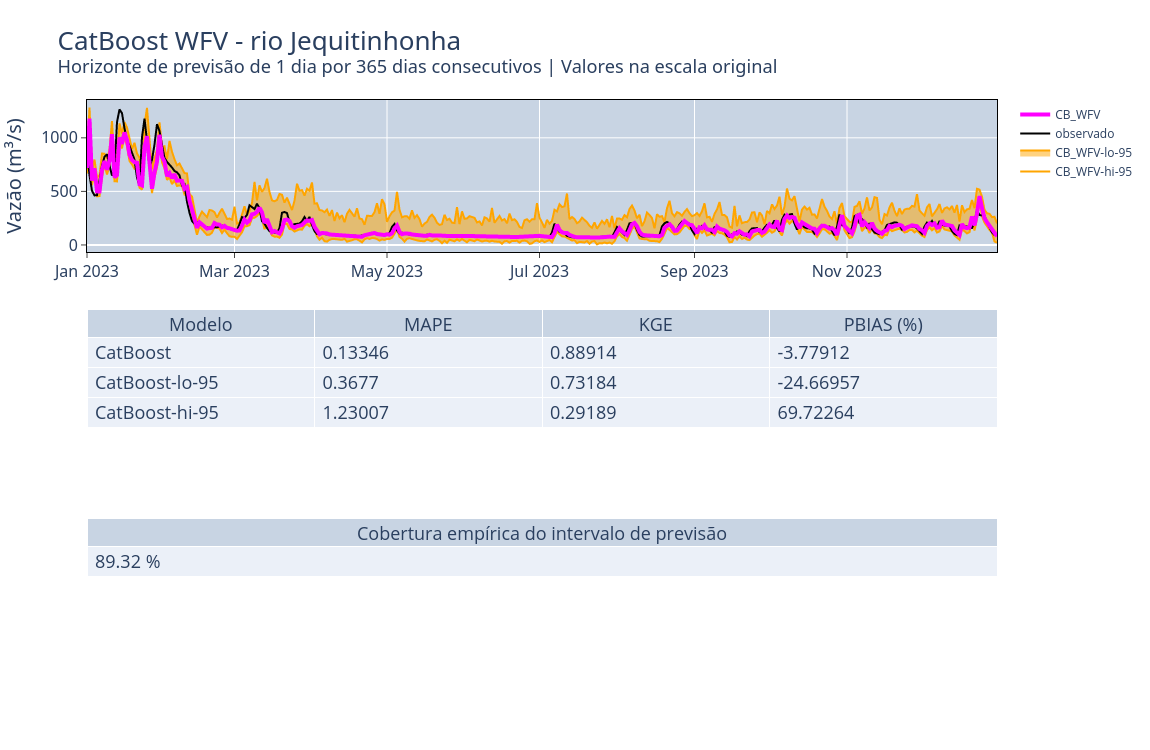
\includegraphics[scale=0.33]{Figuras/jequiti/wfv/CB/CB_WFV_ORIG.png}
\caption{\textit{Walk-Forward Validation} para o modelo CatBoost - CB.\\(fonte: o autor)}
\label{fig:jequiti_CB_WFV_ORIG}
\end{figure}

\begin{figure}[!h]
\centering
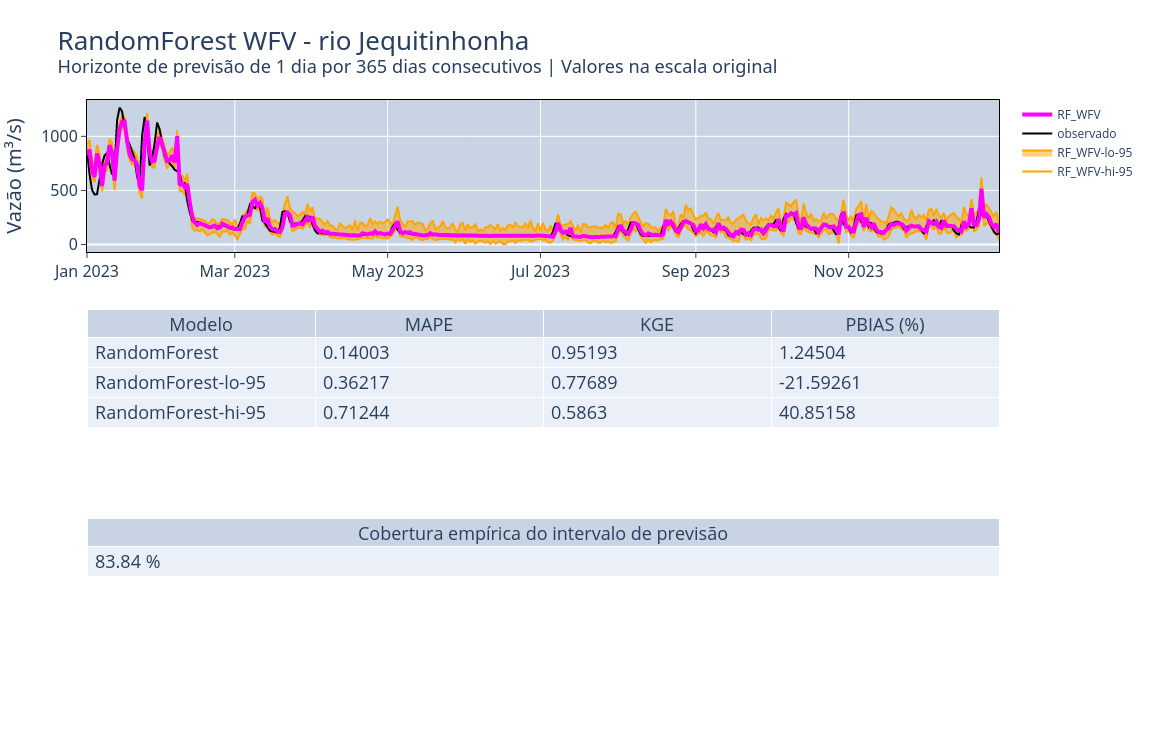
\includegraphics[scale=0.33]{Figuras/jequiti/wfv/RF/RF_WFV_ORIG.png}
\caption{\textit{Walk-Forward Validation} para o modelo RandomForest - RF.\\(fonte: o autor)}
\label{fig:jequiti_RF_WFV_ORIG}
\end{figure}
\clearpage

Observa-se que a maior parte dos resíduos está concentrada em torno da linha de referência $y=0$, o que indica que os modelos CatBoost foram capazes de produzir previsões relativamente boas para a maioria dos dados. Ambos apresentaram também valores extremos, \textit{outliers}, e essa presença pode indicar que os modelos enfrentaram dificuldades em prever corretamente alguns valores mais extremos, resultando em erros maiores para certas previsões. O modelo RF apresenta uma distribuição de resíduos um pouco mais ampla que o CB, com alguns pontos chegando a resíduos superiores a $400$ e abaixo de $-300$.

Ambos os modelos apresentaram bom desempenho geral, com a maioria dos resíduos concentrados em torno da linha de $y=0$, indicando previsões razoáveis. No entanto, também apresentaram \textit{outliers} e tendência dos resíduos aumentarem em magnitude para previsões maiores. Isso indica que tanto o modelo CB quanto o RF podem enfrentar dificuldades em prever valores extremos com precisão, um comportamento já demonstrado anteriormente.

\begin{figure}[!h]
\centering
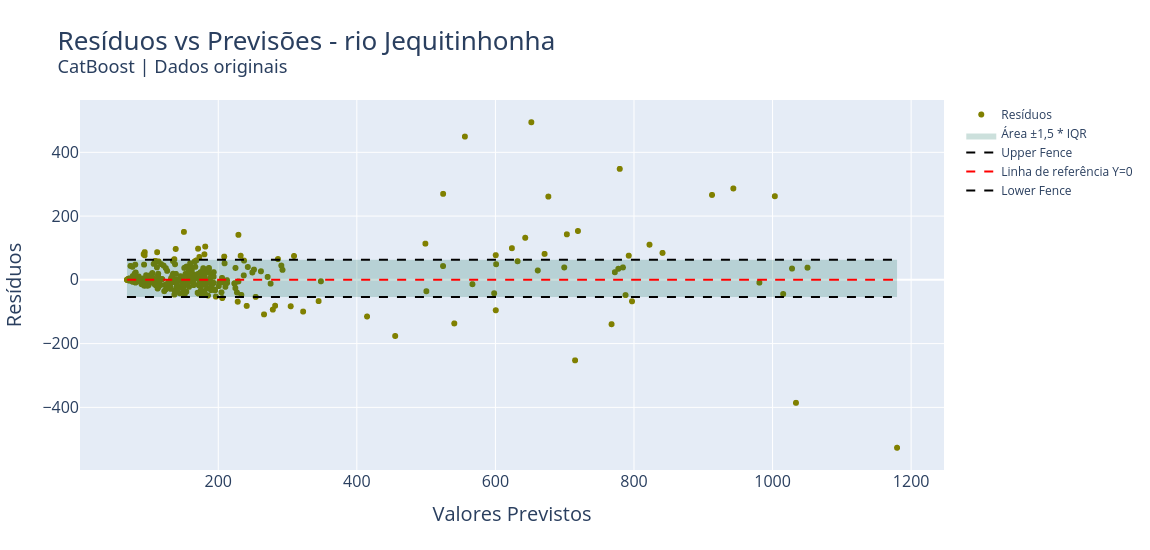
\includegraphics[scale=0.33]{Figuras/jequiti/wfv/CB/CB_WFV_ORIG_RESID_x_PREV.png}
\caption{Dispersão dos resíduos.\\(fonte: o autor)}
\label{fig:jequiti_CB_WFV_ORIG_RESID_x_PREV}
\end{figure}

\begin{figure}[!h]
\centering
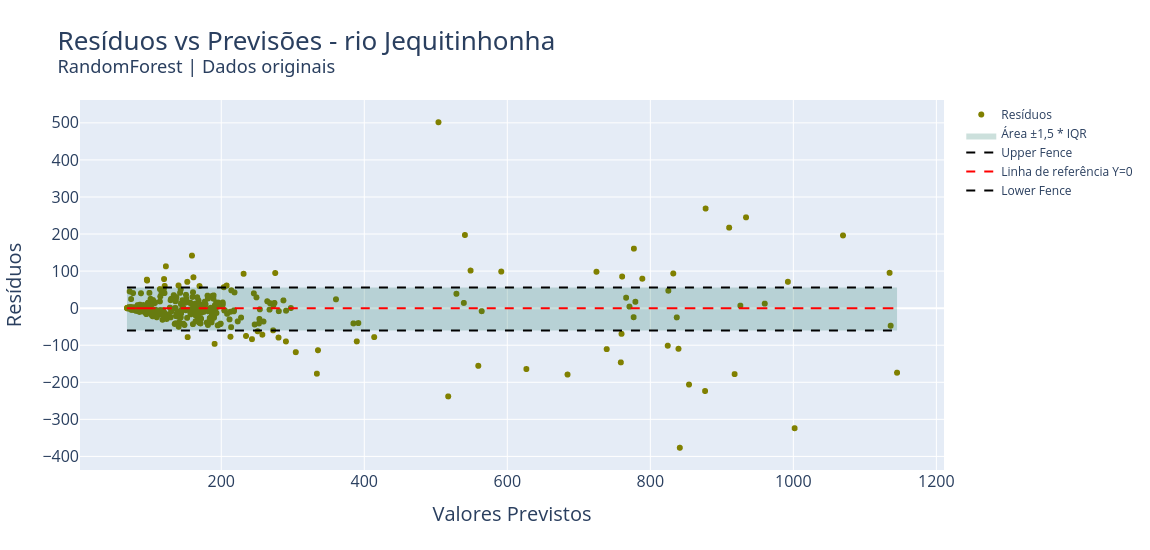
\includegraphics[scale=0.33]{Figuras/jequiti/wfv/RF/RF_WFV_ORIG_RESID_x_PREV.png}
\caption{Dispersão dos resíduos.\\(fonte: o autor)}
\label{fig:jequiti_RF_WFV_ORIG_RESID_x_PREV}
\end{figure}
\clearpage

A maior parte dos resíduos está concentrada em torno da linha de referência $y=0$, indicando que os modelos mantiveram um desempenho geral estável ao longo do tempo. Porém, há \textit{outliers} significativos no início de 2023 (valores de resíduos acima de $400$ e abaixo de $-400$ para o CB e acima de $500$ e abaixo de $-300$ para o RF). Esses outliers indicam que, durante o início do ano, ambos tiveram dificuldades em prever alguns eventos específicos, resultando em erros grandes.

Para o modelo CB, após fevereiro de 2023 (março para o modelo RF), os resíduos parecem estar melhor distribuídos dentro da faixa delimitada pelas faixas, com menos \textit{outliers} extremos, sugerindo que os modelos ajustaram-se melhor aos dados ao longo do tempo.

Em geral, ambos os modelos apresentaram um padrão de melhora ao longo do ano, com resíduos mais bem distribuídos após o primeiro trimestre de 2023. No entanto, os \textit{outliers} iniciais indicam que os modelos podem ter dificuldades com eventos específicos de sazonalidade ou anomalias no início do ano. O CB parece ter uma leve vantagem em termos de previsões mais consistentes ao longo do tempo (valores menos extremos). Ajustes de hiperparâmetros podem ajudar os modelos nos períodos mais desafiadores do ano, como no início do ano, ou adição de componentes de tendência e sazonalidade localizada.

\begin{figure}[!h]
\centering
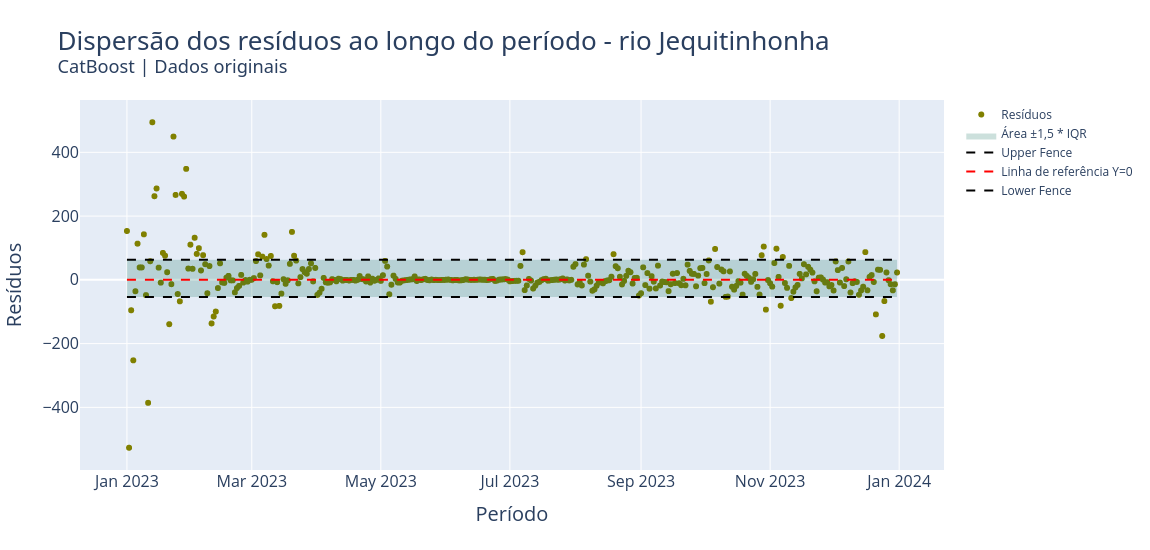
\includegraphics[scale=0.33]{Figuras/jequiti/wfv/CB/CB_WFV_ORIG_RESID_x_TEMPO.png}
\caption{Dispersão dos resíduos ao longo do ano.\\(fonte: o autor)}
\label{fig:jequiti_CB_WFV_ORIG_RESID_x_TEMPO}
\end{figure}

\begin{figure}[!h]
\centering
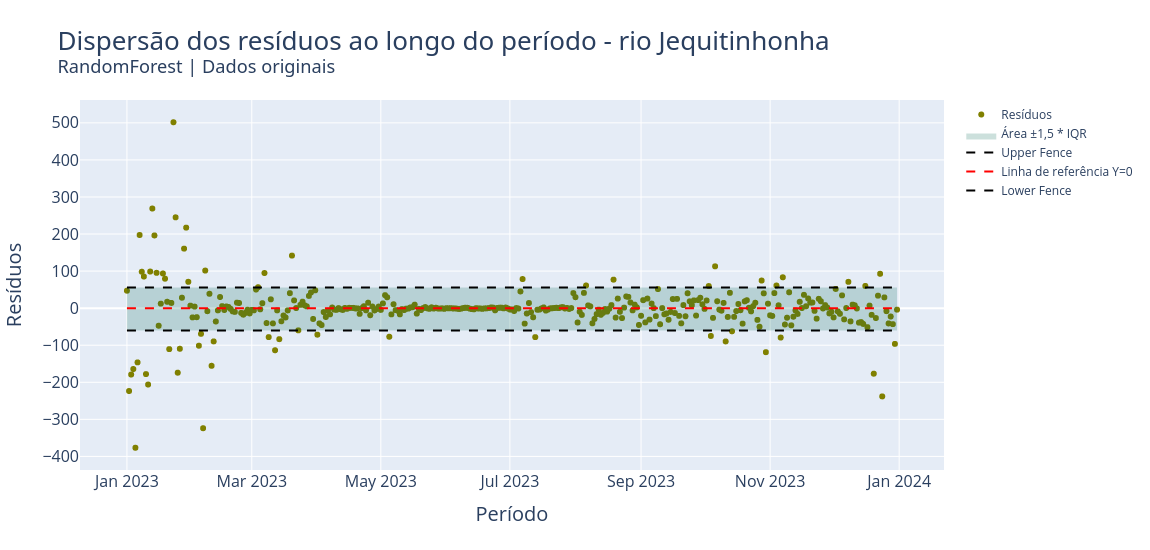
\includegraphics[scale=0.33]{Figuras/jequiti/wfv/RF/RF_WFV_ORIG_RESID_x_TEMPO.png}
\caption{Dispersão dos resíduos ao longo do ano.\\(fonte: o autor)}
\label{fig:jequiti_RF_WFV_ORIG_RESID_x_TEMPO}
\end{figure}
\clearpage

A distribuição dos resíduos do modelo CB (figura \ref{fig:jequiti_CB_WFV_ORIG_RESID_x_CURVA_NORMAL}) apresenta uma assimetria positiva de $1,33$, o que indica que a cauda direita da distribuição é mais longa que a esquerda. Isso significa que há um maior número de resíduos positivos mais elevados (erros positivos grandes) do que negativos. A curva normal ajustada (em vermelho) não se ajusta perfeitamente à distribuição observada, especialmente nas caudas, o que indica que a distribuição dos resíduos não é perfeitamente normal. Esse comportamento é esperado, dado o valor da assimetria. A maior parte dos resíduos está concentrada em torno de $y=0$, com uma contagem elevada próxima a zero. Isso é um bom sinal, pois sugere que o modelo fez previsões razoavelmente precisas para a maior parte dos dados.
No entanto, a presença de resíduos elevados tanto na cauda direita (acima de $200$) quanto na cauda esquerda (abaixo de $-100$) indica que o modelo teve dificuldades em prever com precisão alguns valores mais extremos. A distribuição assimétrica com cauda longa à direita indica que o modelo CB teve mais dificuldades com previsões que resultaram em grandes erros positivos. Esses erros podem ser atribuídos a eventos atípicos ou extremos nos dados, que o modelo não conseguiu prever corretamente.

A distribuição dos resíduos do modelo RF (\ref{fig:jequiti_RF_WFV_ORIG_RESID_x_CURVA_NORMAL}) apresenta uma assimetria positiva de $0,49$, o que indica que a cauda direita é um pouco mais longa, mas a assimetria é menos pronunciada do que no modelo CB. A curva normal ajustada se aproxima mais da distribuição observada do que no gráfico do CB, o que sugere que os resíduos do RF seguem uma distribuição mais próxima de uma normal, apesar da pequena assimetria positiva. Assim como no gráfico do CB, a maior parte dos resíduos está concentrada em torno de zero, com a maioria das previsões sendo razoavelmente precisas. No entanto, o RF apresenta uma distribuição ligeiramente mais equilibrada, com menos resíduos extremos do que o CB. As caudas, tanto à esquerda quanto à direita, são menos pronunciadas, com menos resíduos extremos (acima de $200$ e abaixo de $-200$). Isso indica que o RF teve um desempenho mais estável e com menos erros em eventos extremos.

O RF tem um comportamento de resíduos mais próximo de uma distribuição normal, com menos assimetria e menos resíduos extremos. Isso indica que o modelo é mais estável e robusto em termos de previsões para a maioria dos dados. O CB mostrou maior sensibilidade a eventos extremos, com resíduos mais dispersos e uma assimetria maior, indicando que o modelo enfrenta dificuldades em capturar corretamente os valores mais extremos, resultando em erros maiores. Mas em geral, ambos os modelos apresentam uma boa concentração de resíduos em torno de zero, mostrando que a maioria das previsões está correta, ainda que o CB tenha se apresentado mais suscetível a \textit{outliers}.

\begin{figure}[!h]
\centering
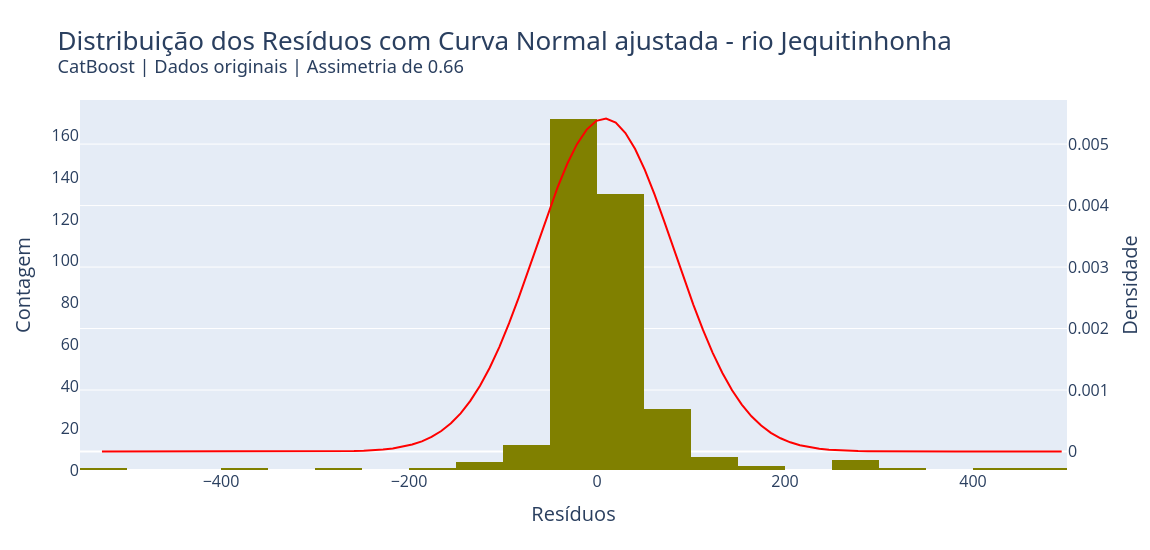
\includegraphics[scale=0.33]{Figuras/jequiti/wfv/CB/CB_WFV_ORIG_RESID_x_CURVA_NORMAL.png}
\caption{Histograma e curva-normal dos resíduos.\\(fonte: o autor)}
\label{fig:jequiti_CB_WFV_ORIG_RESID_x_CURVA_NORMAL}
\end{figure}

\begin{figure}[!h]
\centering
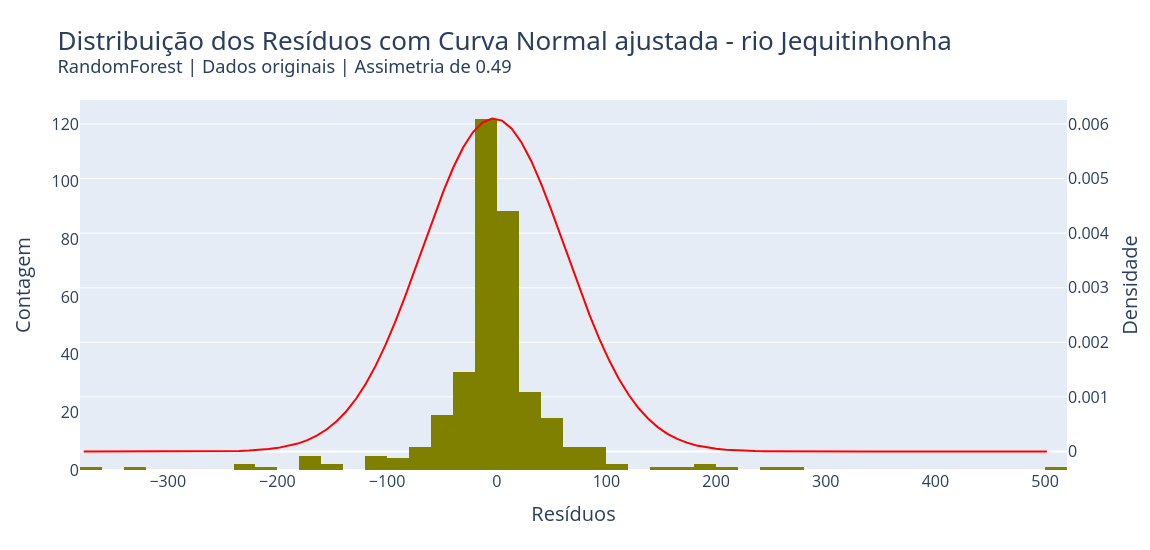
\includegraphics[scale=0.33]{Figuras/jequiti/wfv/RF/RF_WFV_ORIG_RESID_x_CURVA_NORMAL.png}
\caption{Histograma e curva-normal dos resíduos.\\(fonte: o autor)}
\label{fig:jequiti_RF_WFV_ORIG_RESID_x_CURVA_NORMAL}
\end{figure}
\clearpage

Nas primeiras \textit{lags}, há autocorrelações significativas que ultrapassam a faixa de confiança, especialmente nas primeiras 10 \textit{lags}. Isso indica que, para curtos intervalos de tempo, os resíduos do modelo CB estão correlacionados, sugerindo que o modelo deixou de capturar padrões de curto prazo.(figura \ref{fig:jequiti_CB_WFV_ORIG_RESID_ACF}) A presença dessas correlações positivas nos primeiros lags pode sugerir que há padrões temporais nos dados que o modelo CB não capturou adequadamente. No entanto, a partir de aproximadamente a \textit{lag} 20, as autocorrelações caem para valores dentro da faixa de confiança de $95\%$ e permanecem próximas de zero. Isso sugere que, para intervalos maiores, os resíduos não apresentam correlação significativa, o que é um sinal positivo de que, em termos de longo prazo, o modelo está capturando a variabilidade dos dados de forma satisfatória.

Assim como no gráfico do CB, o modelo RF também apresenta autocorrelações significativas nas primeiras \textit{lags} (até cerca de 10 \textit{lags}).(figura \ref{fig:jequiti_RF_WFV_ORIG_RESID_ACF}) Isso indica uma dependência temporal de curto prazo que o modelo RF não capturou completamente, resultando em resíduos correlacionados em intervalos curtos. No entanto, as correlações significativas parecem ser um pouco mais dispersas em comparação com o modelo CB, o que pode indicar um comportamento ligeiramente melhor para curtos intervalos no modelo RF. A partir de aproximadamente a \textit{lag} 20, as autocorrelações do RF caem para dentro da faixa de confiança e permanecem próximas de zero, assim como no modelo CB, indicando que, para previsões de longo prazo, o modelo RF está capturando bem a estrutura dos dados e os resíduos se comportam de maneira aleatória.

Ambos os modelos CB e RF apresentam autocorrelações significativas nas primeiras \textit{lags}, denotando que nenhum modelo conseguiu capturar completamente a dependência temporal de curto prazo nos dados. No entanto, o RF teve uma dispersão um pouco menor de correlações significativas em comparação com o CB, o que indica um desempenho ligeiramente melhor no curto prazo.

Para \textit{lags} maiores (acima de 20), tanto o CB quanto o RF apresentaram resíduos que se comportaram de maneira aleatória, com autocorrelações dentro da faixa de confiança e próximas de zero. Considernado as previsões de longo prazo, ambos os modelos estão funcionando de forma satisfatória e não apresentaram padrões remanescentes nos resíduos.

\begin{figure}[!h]
\centering
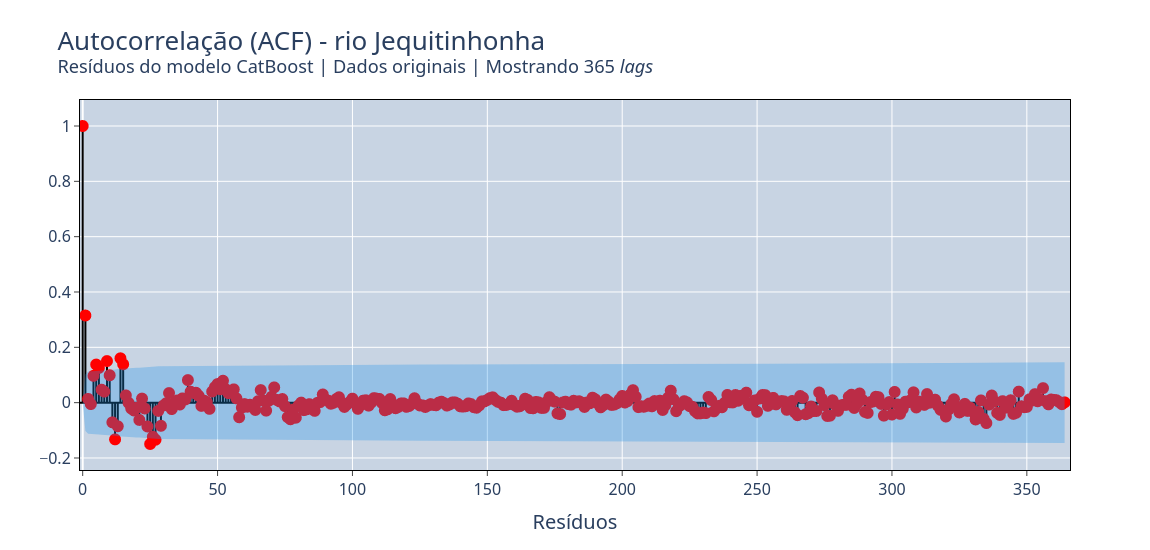
\includegraphics[scale=0.33]{Figuras/jequiti/wfv/CB/CB_WFV_ORIG_RESID_ACF.png}
\caption{Gráfico ACF dos resíduos.\\(fonte: o autor)}
\label{fig:jequiti_CB_WFV_ORIG_RESID_ACF}
\end{figure}

\begin{figure}[!h]
\centering
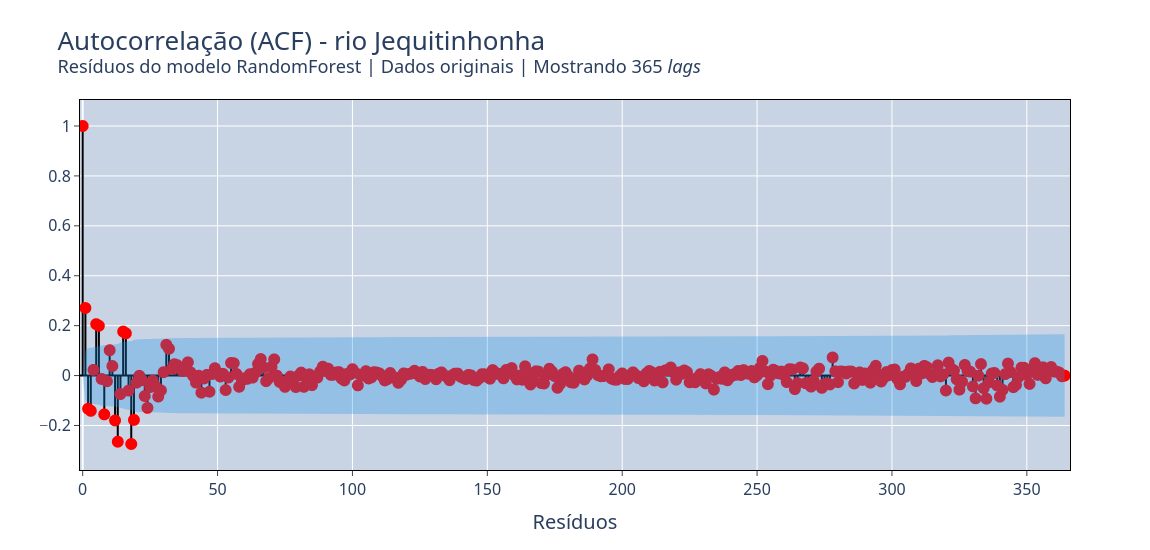
\includegraphics[scale=0.33]{Figuras/jequiti/wfv/RF/RF_WFV_ORIG_RESID_ACF.png}
\caption{Gráfico ACF dos resíduos.\\(fonte: o autor)}
\label{fig:jequiti_RF_WFV_ORIG_RESID_ACF}
\end{figure}
\clearpage

Para o rio Jequitinhonha a análise termina aqui. Aplicar a log-transformação melhorou o resultado do modelo LR de quando não aplicada essa transformação, e os modelos CB e RF (não-lineares) foram melhores quando os dados não foram transformados. Aqui, para este rio, foi este o resultado, mais adiante será visto para os demais rios.

Uma coisa que precisa ficar claro aqui: só serão discutidos para os outros rios os melhores resultados. Para o Jequitinhonha foi mostrada toda linha de trabalho para que ficasse claro que toda comparação foi realizada entre resultados log-transformados e não transformados, tudo foi estudado e analisado. Mas pelo bem da concisão (e deve ter ficado evidente as voltas dadas no texto mostrando exatamente cada resultado), todo resultado não mostrado neste capítulo será colocado em um apêndice para que o leitor e a leitora possam averiguar a corretude do trabalho. E não será mais incluída a análise para o modelo SeasonalNaive.

Adiante.

\subsection{Rio Doce}

Os resultados para o rio Doce apresentaram-se muito bons, considerando-se todas as métricas do trabalho. Isso possivelmente se deve à qualidade dos dados de treinamento, em que não foi preciso preencher tantos dados faltantes de vazão. Relembre: de 4017 registros, apenas 3 faltavam.

O modelo CB apresentou um desempenho muito bom, com a KGE de $0,89$ sugerindo alta correlação entre os valores previstos e os observados. Quando se observa a MAPE, foi a mais baixa entre os três modelos, indicando uma precisão elevada nas previsões, o que demonstra robustez do modelo. A PBIAS de $-3.73\%$ indica um leve viés geral para subestimar as previsões, e a cobertura empírica de $91,23\%$ mostra que o intervalo de previsão captura bem a variabilidade dos dados observados.

O gráfico revela ainda que o modelo acompanha bem os picos de vazão e que os intervalos de previsão foram particularmente estreitos quando no período de vazões elevadas e relativamente amplos nos períodos de menores vazões. Ao que parece, as medições de precipitação nos períodos chuvosos conferem mais precisão ao comportamento médio do modelo. Em outras palavras: o modelo fica mais ``otimista'' quando os dados de chuva não estão zerados, o que ocorre nos períodos de outono e inverno. Tanto que nestes períodos mencionados, quando há uma profusão de valores $0$ na precipitação, os intervalos de previsão ficaram amplos, o que indica a tentativa do modelo de ``acertar'' a medida. Comportamento este que o modelo RF também apresentou em relação aos intervalos de previsão. A cobertura empírica dos intervalos de previsão de ambos os modelos ficaram próximas, com uma leve vantagem para o modelo CB - o modelo RF obteve $88,77\%$. (figuras \ref{fig:doce_CB_WFV_ORIG} e \ref{fig:doce_RF_WFV_ORIG})

O modelo LR, mesmo sendo um modelo simples, apresentou um desempenho notável, com uma MAPE ligeiramente maior, de $0,084$ do que o do CatBoost, mas ainda assim baixo. O KGE foi o maior dos três modelos, alcançando $0,94$, o que indica uma ótima correlação e menor erro de variância. O PBIAS de $-2,75\%$ sugere um viés de subestimação, mas é o menor viés dentre os modelos. A cobertura empírica de $96,71\%$ mostra que o intervalo de confiança captura quase a totalidade da variabilidade dos dados observados.

O gráfico também mostra que a regressão linear consegue capturar os picos de vazão de forma eficaz, com intervalos de confiança mais apertados comparados ao CatBoost.

O modelo RandomForest também teve um bom desempenho, com um MAPE intermediário entre os outros dois modelos e um KGE de $0,93$, o que é muito próximo ao da regressão linear. O PBIAS de $-1,44\%$ indica o menor viés de subestimação entre os três modelos. No entanto, a cobertura empírica foi a menor, com $88,77\%$, sugerindo que o intervalo de confiança não abrange tanto a variabilidade observada quanto nos outros modelos.

No gráfico, os picos de vazão são bem capturados, com um comportamento semelhante ao do CatBoost em termos de previsões.

**Comparação Geral**
- **Precisão (MAPE)**: O CatBoost apresentou o melhor desempenho (0.08207), seguido de perto por RandomForest (0.08355) e LinearRegression (0.08434). A diferença é muito pequena, mostrando que todos os modelos têm alta precisão.

- **Kling-Gupta Efficiency (KGE)**: O modelo de Regressão Linear foi o melhor nesse critério, com 0.94579, seguido pelo RandomForest (0.9375) e o CatBoost (0.8933). Isso sugere que, apesar de ser um modelo linear, a regressão conseguiu capturar bem a dinâmica não-linear das vazões do rio.

- **Bias (\%)**: Todos os modelos apresentaram um leve viés de subestimação, com RandomForest (-1.44\%) sendo o mais equilibrado, seguido por LinearRegression (-2.75\%) e CatBoost (-3.73\%).

- **Intervalos de Confiança**: O CatBoost teve a maior amplitude nos intervalos de confiança, enquanto a regressão linear apresentou os intervalos mais estreitos. Isso se reflete nas coberturas empíricas: a LinearRegression cobre 96.71\% da variabilidade, enquanto o CatBoost cobre 91.23\% e o RandomForest 88.77\%.

**Conclusão**
No geral, todos os três modelos apresentam bons resultados, mas com características específicas:
- O **CatBoost** é ligeiramente melhor em precisão, mas com intervalos de confiança mais amplos e um viés de subestimação mais acentuado.
- A **Regressão Linear** surpreendentemente teve o melhor desempenho no **KGE**, menor viés e a maior cobertura empírica, o que demonstra que pode ser uma alternativa interessante mesmo para dados não transformados.
- O **RandomForest** é competitivo em precisão e viés, mas com uma menor cobertura empírica, sugerindo que os intervalos de confiança são menos eficazes para capturar a incerteza nas previsões.

A escolha do modelo pode depender do equilíbrio entre precisão, viés e a capacidade de capturar a variabilidade dos dados observados, com a regressão linear se mostrando surpreendentemente forte para esse conjunto de dados.

\begin{figure}[!h]
\centering
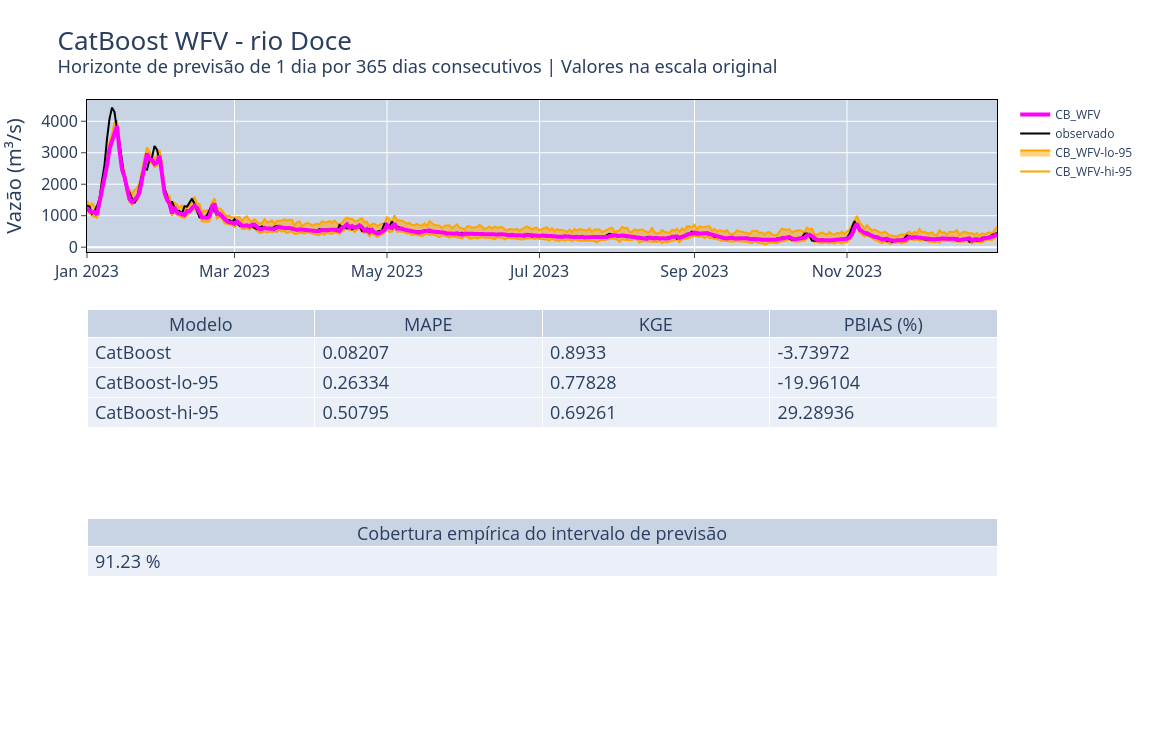
\includegraphics[scale=0.33]{Figuras/rio_doce/wfv/CB/CB_WFV_ORIG.png}
\caption{\textit{Walk-Forward Validation} para o modelo CatBoost - CB.\\(fonte: o autor)}
\label{fig:doce_CB_WFV_ORIG}
\end{figure}

\begin{figure}[!h]
\centering
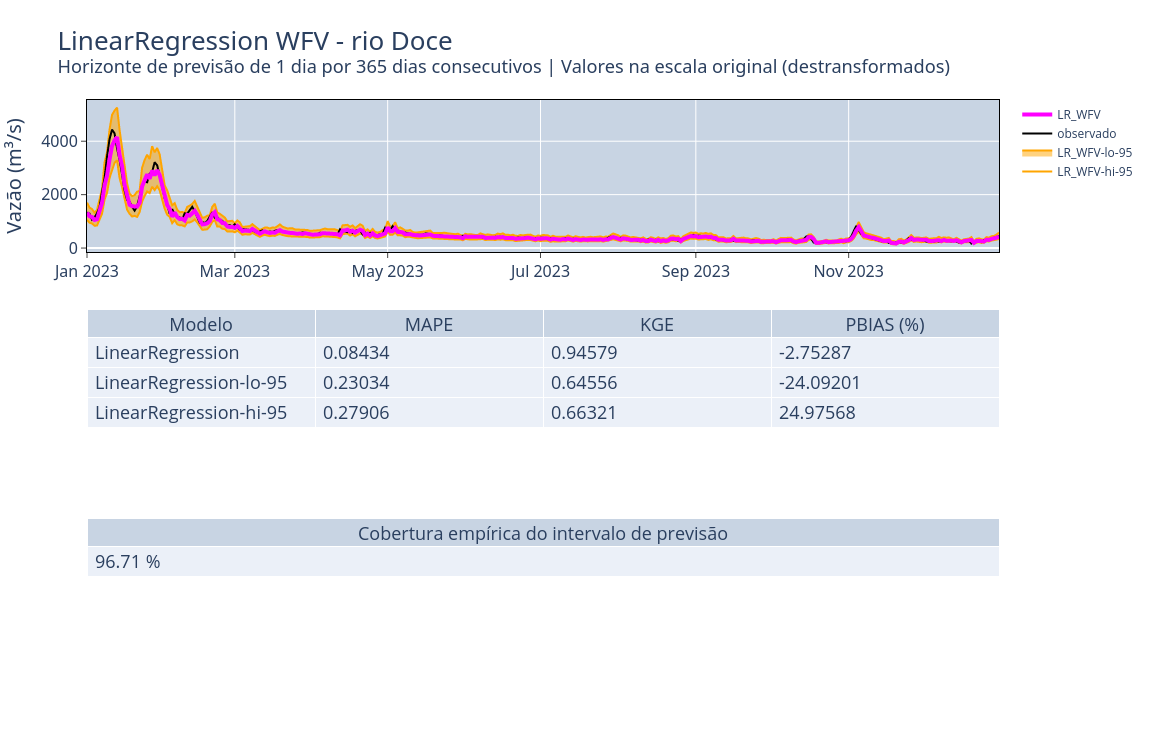
\includegraphics[scale=0.33]{Figuras/rio_doce/wfv/LR/LR_WFV_LOG.png}
\caption{\textit{Walk-Forward Validation} para o modelo LinearRegression - LR.\\(fonte: o autor)}
\label{fig:doce_LR_WFV_LOG}
\end{figure}

\begin{figure}[!h]
\centering
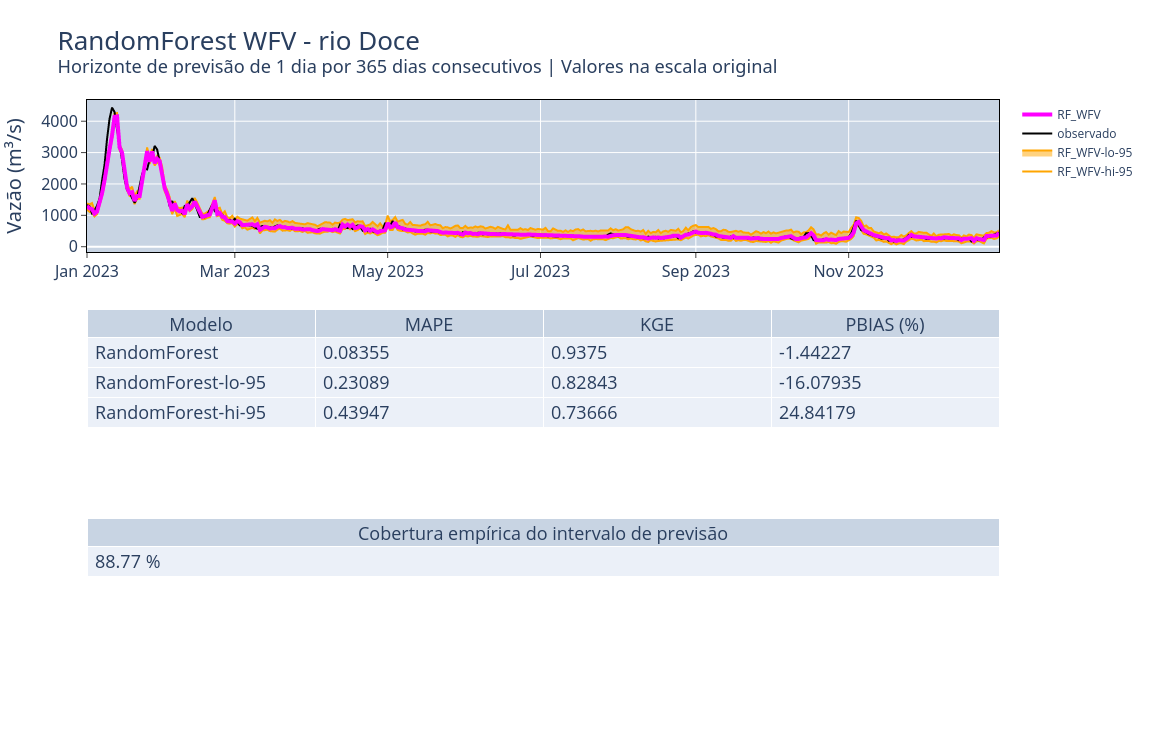
\includegraphics[scale=0.33]{Figuras/rio_doce/wfv/RF/RF_WFV_ORIG.png}
\caption{\textit{Walk-Forward Validation} para o modelo RandomForest - RF.\\(fonte: o autor)}
\label{fig:doce_RF_WFV_ORIG}
\end{figure}
\clearpage

A análise dos gráficos de resíduos para os três modelos (CatBoost, Regressão Linear e RandomForest) ajuda a avaliar o comportamento dos erros das previsões em função dos valores previstos. Vou destacar as características e interpretações para cada um deles:

1. **CatBoost**
- **Padrão dos Resíduos**: O gráfico mostra uma concentração de resíduos em torno de 0 para previsões de até aproximadamente 500 \(m^3/s\), o que indica que o modelo está prevendo bem para valores mais baixos de vazão. No entanto, à medida que os valores previstos aumentam, os resíduos começam a se espalhar mais, o que indica que o modelo tem uma maior dificuldade em capturar picos de vazão mais altos.
- **Outliers**: Existem alguns resíduos que excedem os limites de 1,5 IQR (Interquartile Range), especialmente para previsões mais altas, com resíduos acima de 100 e abaixo de -200, sugerindo a presença de outliers em picos de vazão.
- **Tendência**: Não parece haver uma tendência clara nos resíduos, o que é positivo, pois indica que o modelo não está sistematicamente superestimando ou subestimando em uma faixa específica de valores previstos.

2. **LinearRegression**
- **Padrão dos Resíduos**: Para a Regressão Linear, observa-se um comportamento semelhante ao do CatBoost no que se refere à concentração de resíduos em torno de 0 para valores previstos mais baixos. Contudo, a dispersão dos resíduos é ligeiramente maior para previsões acima de 1000 \(m^3/s\), indicando uma leve perda de precisão em valores mais altos.
- **Outliers**: O modelo de Regressão Linear também mostra alguns outliers em valores previstos mais altos, especialmente entre 2500 e 4000 \(m^3/s\). Isso é esperado, dado que a regressão linear pode ter dificuldades em capturar não-linearidades e picos extremos de vazão.
- **Tendência**: Assim como no CatBoost, não há uma tendência evidente, o que significa que o modelo está relativamente bem ajustado, mas com uma dispersão maior à medida que os valores previstos aumentam.

3. **RandomForest**
- **Padrão dos Resíduos**: O RandomForest apresenta um padrão semelhante ao do CatBoost e da Regressão Linear. A concentração dos resíduos em torno de 0 para previsões menores também está presente, mas há uma maior dispersão dos resíduos para previsões acima de 1000 \(m^3/s\). Isso indica que, assim como os outros modelos, o RandomForest tem dificuldade em capturar corretamente os picos mais altos de vazão.
- **Outliers**: Notam-se outliers para valores previstos mais altos, com resíduos que variam de 300 a mais de 1000 para previsões maiores que 2500 \(m^3/s\). Esses outliers são mais pronunciados que nos outros dois modelos.
- **Tendência**: Novamente, não há uma tendência clara nos resíduos, mas a dispersão dos erros aumenta com os valores previstos, indicando que o modelo perde precisão nos valores de pico.

**Comparação entre os Modelos**
- **Concentração de Resíduos**: Todos os três modelos apresentam uma concentração de resíduos razoavelmente próxima de 0 para valores de vazão previstos abaixo de 1000 \(m^3/s\), sugerindo que eles conseguem modelar bem as vazões mais comuns e de baixa intensidade.
- **Dispersão dos Resíduos**: À medida que os valores previstos aumentam, todos os modelos mostram uma dispersão crescente nos resíduos, com picos de vazão sendo mais difíceis de prever corretamente. Contudo, o **RandomForest** parece ter a maior dispersão, seguido pela **Regressão Linear**, enquanto o **CatBoost** mostra uma dispersão ligeiramente menor, embora ainda presente.
- **Outliers**: Os três modelos possuem outliers, especialmente em previsões mais altas, o que é um desafio típico em dados de vazão de rios, que têm picos esporádicos. O **RandomForest** tem os outliers mais extremos, seguidos pela **Regressão Linear** e, por fim, o **CatBoost**.
- **Tendências**: Nenhum dos modelos apresentou tendências claras de superestimação ou subestimação, o que é positivo. Entretanto, a crescente dispersão dos resíduos em valores previstos mais altos sugere que todos os modelos enfrentam desafios em prever valores de vazão muito elevados.

**Conclusão**
Os três modelos têm desempenho similar em termos de concentração de resíduos para valores baixos de previsão, mas divergem nos valores mais altos. O **CatBoost** se destaca por ter uma menor dispersão de resíduos em previsões elevadas, seguido pela **Regressão Linear**. O **RandomForest** tem a maior dispersão de resíduos e mais outliers, sugerindo que pode não ser a melhor escolha para prever picos extremos de vazão.

\begin{figure}[!h]
\centering
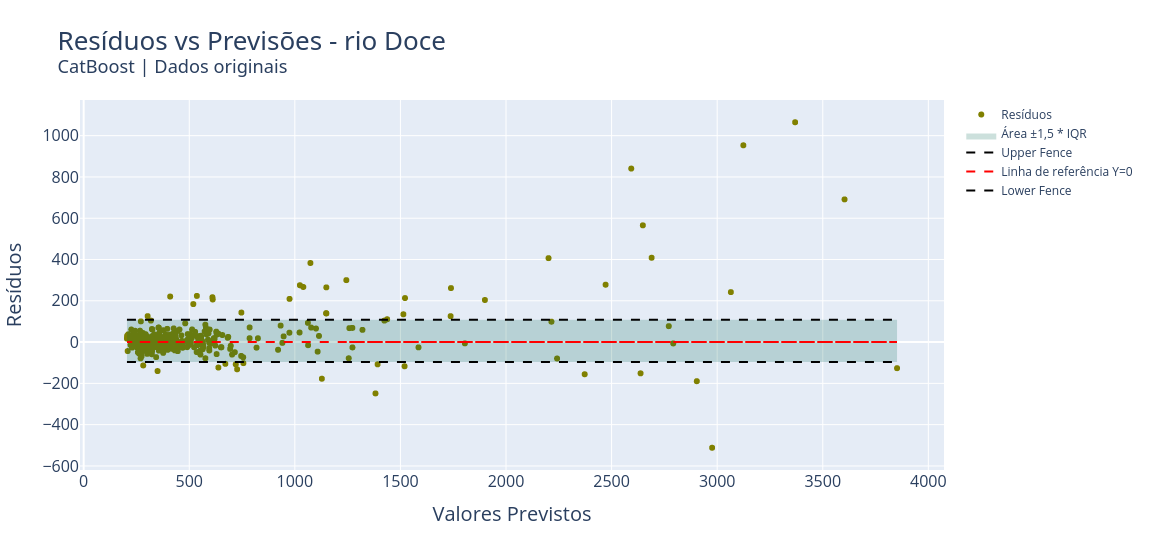
\includegraphics[scale=0.33]{Figuras/rio_doce/wfv/CB/CB_WFV_ORIG_RESID_x_PREV.png}
\caption{Dispersão dos resíduos.\\(fonte: o autor)}
\label{fig:doce_CB_WFV_ORIG_RESID_x_PREV}
\end{figure}

\begin{figure}[!h]
\centering
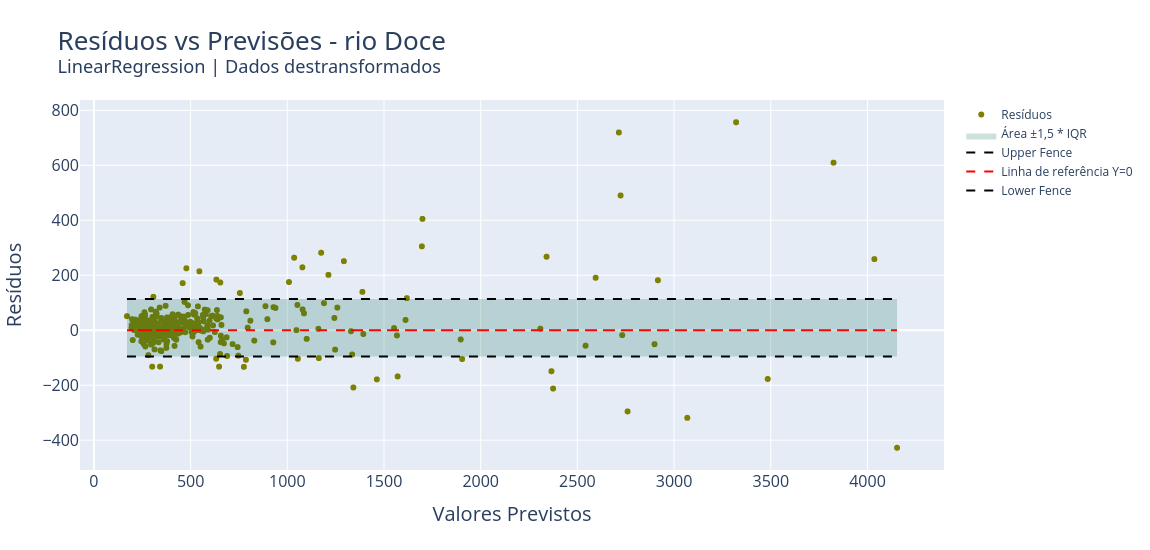
\includegraphics[scale=0.33]{Figuras/rio_doce/wfv/LR/LR_WFV_LOG_RESID_x_PREV.png}
\caption{Dispersão dos resíduos.\\(fonte: o autor)}
\label{fig:doce_LR_WFV_LOG_RESID_x_PREV}
\end{figure}

\begin{figure}[!h]
\centering
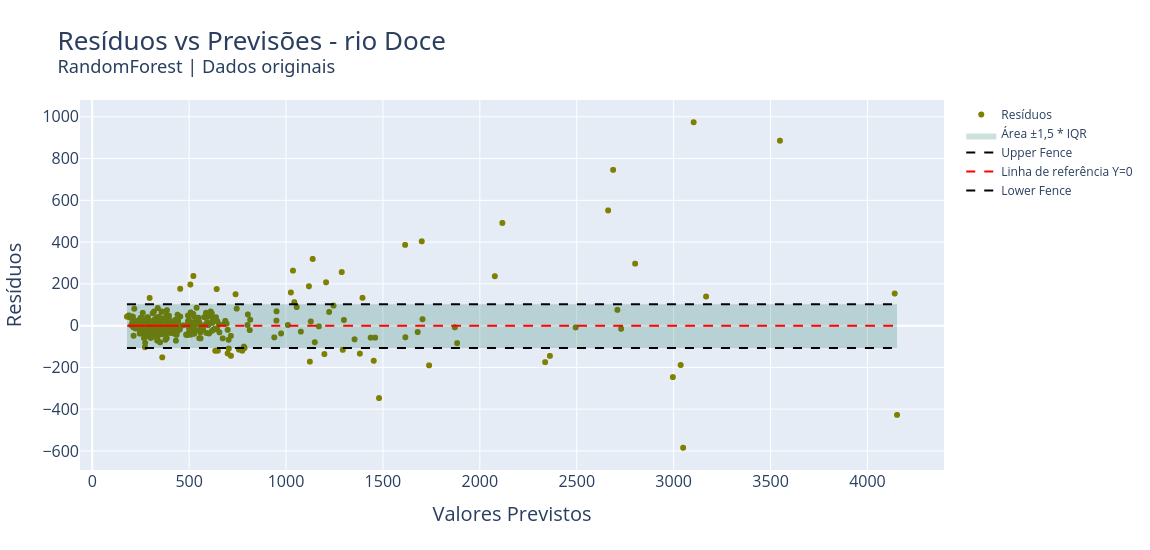
\includegraphics[scale=0.33]{Figuras/rio_doce/wfv/RF/RF_WFV_ORIG_RESID_x_PREV.png}
\caption{Dispersão dos resíduos.\\(fonte: o autor)}
\label{fig:doce_RF_WFV_ORIG_RESID_x_PREV}
\end{figure}
\clearpage

\subsection{Rio Grande}

\section{Importância das variáveis}
%Analisar a importância das variáveis contínuas e categóricas na previsão (feature importance).

\section{Discuss\~ao dos resultados}
%Interpretar os resultados e discutir as limitações. Se possível, comparar com estudos anteriores.